%%%%%%%%%%%%%%%%%%%%%%%%%%%%%%%%%%%%%%%%%
% Masters/Doctoral Thesis 
% LaTeX Template
% Version 2.5 (27/8/17)
%
% This template was downloaded from:
% http://www.LaTeXTemplates.com
%
% Version 2.x major modifications by:
% Vel (vel@latextemplates.com)
%
% This template is based on a template by:
% Steve Gunn (http://users.ecs.soton.ac.uk/srg/softwaretools/document/templates/)
% Sunil Patel (http://www.sunilpatel.co.uk/thesis-template/)
%
% Template license:
% CC BY-NC-SA 3.0 (http://creativecommons.org/licenses/by-nc-sa/3.0/)
%
%%%%%%%%%%%%%%%%%%%%%%%%%%%%%%%%%%%%%%%%%

%----------------------------------------------------------------------------------------
%	PACKAGES AND OTHER DOCUMENT CONFIGURATIONS
%----------------------------------------------------------------------------------------

\documentclass[
11pt, % The default document font size, options: 10pt, 11pt, 12pt
oneside, % Two side (alternating margins) for binding by default, uncomment to switch to one side
english,
spanish, % ngerman for German
singlespacing, % Single line spacing, alternatives: onehalfspacing or doublespacing
%draft, % Uncomment to enable draft mode (no pictures, no links, overfull hboxes indicated)
%nolistspacing, % If the document is onehalfspacing or doublespacing, uncomment this to set spacing in lists to single
%liststotoc, % Uncomment to add the list of figures/tables/etc to the table of contents
%toctotoc, % Uncomment to add the main table of contents to the table of contents
parskip, % Uncomment to add space between paragraphs
%nohyperref, % Uncomment to not load the hyperref package
headsepline, % Uncomment to get a line under the header
%chapterinoneline, % Uncomment to place the chapter title next to the number on one line
%consistentlayout, % Uncomment to change the layout of the declaration, abstract and acknowledgements pages to match the default layout
]{MastersDoctoralThesis} % The class file specifying the document structure

%\usepackage[english,spanish]{babel}
\usepackage[utf8]{inputenc} % Required for inputting international characters
\usepackage[T1]{fontenc} % Output font encoding for international characters

\usepackage{mathpazo} % Use the Palatino font by default

\usepackage{float}

\usepackage[backend=bibtex,style=numeric-comp,natbib=true]{biblatex} % Use the bibtex backend with the authoryear citation style (which resembles APA)

\addbibresource{bibliography.bib} % The filename of the bibliography

\usepackage[autostyle=true]{csquotes} % Required to generate language-dependent quotes in the bibliography

%\usepackage{hyperref}

%--------------------------------------------
% Listing for JavaScript
%--------------------------------------------

\usepackage{listings}
\usepackage{color}
\definecolor{antiflash-white}{rgb}{0.95, 0.95, 0.96}
\definecolor{super-gray}{rgb}{0.98, 0.98, 0.98}
\definecolor{darkgray}{rgb}{.4,.4,.4}
\definecolor{purple}{rgb}{0.65, 0.12, 0.82}

\lstdefinelanguage{JavaScript}{
  keywords={typeof, new, true, false, catch, function, return, null, catch, switch, var, if, in, while, do, else, case, break, for, let, const},
  keywordstyle=\color{blue}\bfseries,
  ndkeywords={class, export, boolean, throw, implements, import, this, extends, super, default, from},
  ndkeywordstyle=\color{darkgray}\bfseries,
  identifierstyle=\color{black},
  sensitive=false,
  comment=[l]{//},
  morecomment=[s]{/*}{*/},
  commentstyle=\color{purple}\ttfamily,
  stringstyle=\color{red}\ttfamily,
  morestring=[b]',
  morestring=[b]"
}


\lstset{
   language=JavaScript,
   backgroundcolor=\color{antiflash-white},
   extendedchars=true,
   basicstyle=\footnotesize\ttfamily,
   showstringspaces=false,
   showspaces=false,
   numbers=left,
   numberstyle=\footnotesize,
   numbersep=10pt,
   tabsize=2,
   breaklines=true,
   showtabs=false,
   captionpos=b,
	 frame=top,
	 frame=bottom
}




%----------------------------------------------------------------------------------------
%	MARGIN SETTINGS
%----------------------------------------------------------------------------------------

\geometry{
	paper=a4paper, % Change to letterpaper for US letter
	inner=2.5cm, % Inner margin
	outer=3cm, % Outer margin //  outer=3.8cm
	bindingoffset=.5cm, % Binding offset
	top=1.5cm, % Top margin
	bottom=1.5cm, % Bottom margin
	%showframe, % Uncomment to show how the type block is set on the page
}

%----------------------------------------------------------------------------------------
%	THESIS INFORMATION
%----------------------------------------------------------------------------------------

\thesistitle{JavaScript: Lo bueno, lo malo y lo feo} % Your thesis title, this is used in the title and abstract, print it with \ttitle
\supervisor{Dra. María Laura \textsc{Cobo}\\Dr. Sebastián \textsc{Gottifredi}} % Your supervisor's name, this is used in the title page, print it elsewhere with \supname
\examiner{} % Your examiner's name, this is not currently used anywhere in the template, print it elsewhere with \examname
\degree{Licenciatura en Ciencias de la Computación} % Your degree name, this is used in the title page and abstract, print it elsewhere with \degreename
\author{Ricardo \textsc{Ferro Moreno}} % Your name, this is used in the title page and abstract, print it elsewhere with \authorname
\addresses{} % Your address, this is not currently used anywhere in the template, print it elsewhere with \addressname

%\subject{Biological Sciences} % Your subject area, this is not currently used anywhere in the template, print it elsewhere with \subjectname
\keywords{} % Keywords for your thesis, this is not currently used anywhere in the template, print it elsewhere with \keywordnames
\university{\href{http://www.uns.edu.ar}{Universidad Nacional del Sur}} % Your university's name and URL, this is used in the title page and abstract, print it elsewhere with \univname
\department{\href{http://cs.uns.edu.ar}{Departamento de Ciencias e Ingeniería de la Computación}} % Your department's name and URL, this is used in the title page and abstract, print it elsewhere with \deptname
\group{\href{http://cs.uns.edu.ar}{UNS}} % Your research group's name and URL, this is used in the title page, print it elsewhere with \groupname
\faculty{\href{http://cs.uns.edu.ar}{UNS}} % Your faculty's name and URL, this is used in the title page and abstract, print it elsewhere with \facname

\AtBeginDocument{
\hypersetup{pdftitle=\ttitle} % Set the PDF's title to your title
\hypersetup{pdfauthor=\authorname} % Set the PDF's author to your name
\hypersetup{pdfkeywords=\keywordnames} % Set the PDF's keywords to your keywords
}

\begin{document}

\frontmatter % Use roman page numbering style (i, ii, iii, iv...) for the pre-content pages

\pagestyle{plain} % Default to the plain heading style until the thesis style is called for the body content

%----------------------------------------------------------------------------------------
%	TITLE PAGE
%----------------------------------------------------------------------------------------

\begin{titlepage}
\begin{center}

\vspace*{.06\textheight}
{\scshape\LARGE Tesis de grado\par} % University name	% \vspace{1.5cm}
\textsc{\Large Licenciatura en Ciencias de la Computación}\\[1.5cm] % Thesis type

\HRule \\[0.4cm] % Horizontal line
{\huge \bfseries \ttitle\par}\vspace{0.4cm} % Thesis title
\HRule \\[0.4cm] % Horizontal line

\begin{minipage}[t]{0.4\textwidth}
\begin{flushleft} \large
\emph{Autor:}\\
{\authorname} % Author name - remove the \href bracket to remove the link
\end{flushleft}
\end{minipage}
\begin{minipage}[t]{0.4\textwidth}
\begin{flushright} \large
\emph{Directores:} \\
{\supname} % Supervisor name - remove the \href bracket to remove the link  
\end{flushright}
\end{minipage}\\[3cm]

\vfill


\includegraphics[scale=0.15]{Logo} % University/department logo - uncomment to place it

%\large \textit{A thesis submitted in fulfillment of the requirements\\ for the degree of \degreename}\\[0.3cm] % University requirement text
%\textit{in the}\\[0.4cm]
\deptname\\\univname\\[1cm] % Research group name and department name


\vfill

{\large \the\year}\\[4cm] % Date
 
\vfill
\end{center}
\end{titlepage}

%----------------------------------------------------------------------------------------
%	DECLARATION PAGE
%----------------------------------------------------------------------------------------

%\begin{declaration}
%\addchaptertocentry{\authorshipname} % Add the declaration to the table of contents
%\noindent I, \authorname, declare that this thesis titled, \enquote{\ttitle} and the work presented in it are my own. I confirm that:

%\begin{itemize} 
%\item This work was done wholly or mainly while in candidature for a research degree at this University.
%\item Where any part of this thesis has previously been submitted for a degree or any other qualification at this University or any other institution, this has been clearly stated.
%\item Where I have consulted the published work of others, this is always clearly attributed.
%\item Where I have quoted from the work of others, the source is always given. With the exception of such quotations, this thesis is entirely my own work.
%\item I have acknowledged all main sources of help.
%\item Where the thesis is based on work done by myself jointly with others, I have made clear exactly what was done by others and what I have contributed myself.\\
%\end{itemize}
 
%\noindent Signed:\\
%\rule[0.5em]{25em}{0.5pt} % This prints a line for the signature
 
%\noindent Date:\\
%\rule[0.5em]{25em}{0.5pt} % This prints a line to write the date
%\end{declaration}

%\cleardoublepage

%----------------------------------------------------------------------------------------
%	QUOTATION PAGE
%----------------------------------------------------------------------------------------

%\vspace*{0.2\textheight}

%\noindent\enquote{\itshape Thanks to my solid academic training, today I can write hundreds of words on virtually any topic without possessing a shred of information, which is how I got a good job in journalism.}\bigbreak

%\hfill Dave Barry

%----------------------------------------------------------------------------------------
%	ABSTRACT PAGE
%----------------------------------------------------------------------------------------

%\begin{abstract}
%\addchaptertocentry{\abstractname} % Add the abstract to the table of contents
%The Thesis Abstract is written here (and usually kept to just this page). The page is kept centered vertically so can expand into the blank space above the title too\ldots
%\end{abstract}

%----------------------------------------------------------------------------------------
%	ACKNOWLEDGEMENTS
%----------------------------------------------------------------------------------------

%\begin{acknowledgements}
%\addchaptertocentry{\acknowledgementname} % Add the acknowledgements to the table of contents
%The acknowledgments and the people to thank go here, don't forget to include your project advisor\ldots
%\end{acknowledgements}

%----------------------------------------------------------------------------------------
%	LIST OF CONTENTS/FIGURES/TABLES PAGES
%----------------------------------------------------------------------------------------

\tableofcontents % Prints the main table of contents

%\listoffigures % Prints the list of figures

%\listoftables % Prints the list of tables

%----------------------------------------------------------------------------------------
%	ABBREVIATIONS
%----------------------------------------------------------------------------------------

%\begin{abbreviations}{ll} % Include a list of abbreviations (a table of two columns)

%\textbf{LAH} & \textbf{L}ist \textbf{A}bbreviations \textbf{H}ere\\
%\textbf{WSF} & \textbf{W}hat (it) \textbf{S}tands \textbf{F}or\\

%\end{abbreviations}

%----------------------------------------------------------------------------------------
%	PHYSICAL CONSTANTS/OTHER DEFINITIONS
%----------------------------------------------------------------------------------------

%\begin{constants}{lr@{${}={}$}l} % The list of physical constants is a three column table

% The \SI{}{} command is provided by the siunitx package, see its documentation for instructions on how to use it

%Speed of Light & $c_{0}$ & \SI{2.99792458e8}{\meter\per\second} (exact)\\
%Constant Name & $Symbol$ & $Constant Value$ with units\\

%\end{constants}

%----------------------------------------------------------------------------------------
%	SYMBOLS
%----------------------------------------------------------------------------------------

%\begin{symbols}{lll} % Include a list of Symbols (a three column table)

%$a$ & distance & \si{\meter} \\
%$P$ & power & \si{\watt} (\si{\joule\per\second}) \\
%Symbol & Name & Unit \\

%\addlinespace % Gap to separate the Roman symbols from the Greek

%$\omega$ & angular frequency & \si{\radian} \\

%\end{symbols}

%----------------------------------------------------------------------------------------
%	DEDICATION
%----------------------------------------------------------------------------------------

%\dedicatory{For/Dedicated to/To my\ldots} 


%----------------------------------------------------------------------------------------
% COMANDOS
%----------------------------------------------------------------------------------------

% Define some commands to keep the formatting separated from the content 
\newcommand{\keyword}[1]{\textbf{#1}}
\newcommand{\tabhead}[1]{\textbf{#1}}
\newcommand{\code}[1]{\texttt{#1}}
\newcommand{\file}[1]{\texttt{\bfseries#1}}
\newcommand{\option}[1]{\texttt{\itshape#1}}
\newcommand{\nuevo}[1]{\fcolorbox{red}{white}{%
    \minipage[t]{\linewidth\fboxsep\fboxrule\relax}
        #1
    \endminipage}}


%----------------------------------------------------------------------------------------
%	THESIS CONTENT - CHAPTERS
%----------------------------------------------------------------------------------------

\mainmatter % Begin numeric (1,2,3...) page numbering

\pagestyle{thesis} % Return the page headers back to the "thesis" style

% Include the chapters of the thesis as separate files from the Chapters folder
% Uncomment the lines as you write the chapters

% INTRO
\chapter{Introducción a la tesis} % Main chapter title

\label{ch:introtesis} % For referencing the chapter elsewhere, use \ref{Chapter1} 

\section{Motivación}

Hay una realidad de la que no se puede escapar, que es que hoy Javascript es uno de los lenguajes más utilizados a nivel empresarial. No solamente eso, sino que gracias a la aparición de Node en 2009, junto con una gran actualización del estandar ECMAScript en 2015 (también conocido como ES6), el lenguaje fue empezado a ser tratado de una forma más seria, abriéndose a nuevos dominios de aplicaciones, donde antes Javascript no era considerado como una posible solución.

Otro detalle, es que Javascript "`ganó"' demasiado terreno siendo el lenguaje pionero para ser implementado en los navegadores, además de que su comunidad ha crecido a un ritmo enorme en los últimos años. A nivel \textit{frontend} en la web, al día de hoy los frameworks más populares usados son React, Angular y Vue, mientras que jQuery se quedó un poco atrás pero sigue en vigencia. Esos cuatro frameworks utilizan Javascript. Por el lado del \textit{backend}, Node también está haciendo lo suyo. No solo eso, sino que además lo expande a otros dominios de aplicación, como pueden ser las aplicaciones de escritorio o la robótica.

Sin embargo es imposible evitar leer críticas del lenguaje, a veces infundadas. Agregando el dato de que la gama de opiniones y críticas es muy amplia, yendo desde el fanatismo del lenguaje hasta el odio profundo. Dicho esto, la motivación de hacer una tesis analizando el lenguaje está atada a los siguientes objetivos:

\begin{itemize}
\item Entender características profundas del lenguaje para comprender qué sucede a bajo nivel.
\item Ganar experiencia en el área. Poder analizar, trazar y debuggear código con facilidad.
\item Corroborar o desmitificar las críticas que se le suelen hacer al lenguaje.
\item Analizar la relación del lenguaje con respecto a los paradigmas de programación populares.
\end{itemize}

\section{Estructura de la tesis}

El documento tiene un capítulo de introducción al lenguaje donde se presentará tanto su historia, como también características subyacentes y conceptos que serán de uso para entender los capítulos siguientes. Luego, la tesis se divide en dos partes: "`Sistema de tipos"' y "`Paradigmas de programación"'. 

En la primera parte se hablará sobre características, debilidades y fortalezas dentro del sistema de tipos del lenguaje. Se hará mención sobre los tipos que tiene el lenguaje y algunas incoherencias sobre los mismos. También se revisarán cuestiones sobre coerción en algunas expresiones, y parte de cómo trabaja el scope del lenguaje.

La segunda parte trata sobre Javascript y los paradigmas de programación, donde se lo evalúa frente al paradigma funcional y el orientado a objetos. Se intentará determinar cuán cercano es el soporte que tiene el lenguaje ante las características de éstos paradigmas.

Cada parte tiene una sección de conclusiones, detallando \textit{lo bueno, lo malo y lo feo} de los temas tratados. No se intenta imponer una opinión como una única verdad, sino más bien acercar al lector mostrando fortalezas y debilidades del lenguaje, para que éste pueda sacar sus propias conclusiones.

La tesis se resume con una conclusión general sobre lo visto, y una breve recopilación sobre conceptos que no han sido tratados en el documento, pero destacables en caso de que el lector quisiera seguir ampliando la investigaciónn.
% Chapter 1

\chapter{Scope} % Main chapter title

\label{ch:scope} % For referencing the chapter elsewhere, use \ref{Chapter1} 



% PARTE 1: Sistema de Tipos
\part{Sistema de Tipos}
\chapter{Tipos} % Main chapter title

\label{ch:tipos} % For referencing the chapter elsewhere, use \ref{Chapter1} 

%----------------------------------------------------------------------------------------

JavaScript es un lenguaje de "`scripting"', con tipado dinámico y un sistema de tipos débil. Generalmente, en este tipo de lenguajes interpretados no es necesario definir el tipo de una variable al momento de declararla. Con tan solo asignarle un valor a esa variable, estamos "`especificando"' su tipo. De hecho, cuando hablamos de tipos, en realidad nos referimos al tipo del valor, y no del identificador de la variable ligado a ese valor.

A veces es necesario \textit{cuestionar} a los tipos que posee un lenguaje para conocerlos mejor. En este capítulo nos aproximaremos a cuestiones relativas a los tipos del lenguaje. Además, se hará un análisis especial del operador \code{typeof}, donde podremos comenzar a observar las flaquezas e incoherencias del lenguaje.

\section{Tipos primitivos}

Tal como se mencionó en el capítulo \ref{ch:introduccionjs}, existen solamente 7 tipos primitivos del lenguaje. Una variable está asociada a un valor, y dicho valor puede ser de alguno de los siguientes tipos:

\begin{itemize}
\item \code{undefined}
\item \code{null}
\item \code{number}
\item \code{string}
\item \code{boolean}
\item \code{symbol}
\item \code{object}
\end{itemize}

Algunos autores consideran que \code{Object} no es un tipo primitivo. De hecho, en la sección \ref{sec:toprimitive} (y a lo largo del capítulo \ref{ch:coercion}) mostraremos que la especificación de ECMAScript \cite{EcmaScript:15} hace una distinción especial para éste a la hora de hacer conversiones de tipo, por lo que pensar que \code{Object} no es un tipo primitivo da lugar a debate, y es un pensamiento totalmente válido.

También existe un concepto errado de que "`en JavaScript todo es un objeto"'. Considerando que en JavaScript las funciones y los arreglos son objetos, la frase es en parte cierta. Pero el concepto es equivocado porque además de objetos existen los otros tipos primitivos, los cuales acabamos de mencionar.

En las siguientes subsecciones haremos introducción (y algunas críticas) a algunos de los tipos. No son tenidos en cuenta \code{boolean}, dado que no hay mucho que analizar, y tampoco \code{symbol}, el cual no formará parte de éste documento.

\subsection{\code{null} y \code{undefined}}

Estos dos tipos representan el valor "`vacío"', y puede resultar confuso, porque tener dos identificadores para \textit{casi} lo mismo parece redundante. El valor de \code{undefined} se suele utilizar como valor para variables que aún no fueron declaradas, mientras que el valor de \code{null} se supone que cuando queremos forzar a que una variable tenga valor nulo.

\begin{lstlisting}[title={\code{null} y \code{undefined}}]
var a;
var b = null;

console.log(a);	// undefined
console.log(b);	// null
\end{lstlisting}

El problema de \code{undefined} es que no existe un mecanismo para restringir el uso de este tipo. De hecho, podemos asignarle \code{undefined} como valor a una variable, y en ese sentido no podemos saber si fue porque se le asignó el valor o porque nunca obtuvo uno.

\begin{lstlisting}
var a;
var b = null;
b = undefined;

console.log(a);	// undefined
console.log(b);	// undefined
\end{lstlisting}

Aquí es donde entra el juego el significado de un valor "`no definido"' y un valor "`no declarado"'. Lo lógico, es pensar que \code{undefined} se utiliza para una variable que sí fue declarada, pero que su valor aún no fue definido. Mientras que una variable "`no declarada"' representaría a una variable que en ningún momento se la declaró mediante ningún mecanismo (ni \code{var}, ni \code{let}, ni \code{const}).

Un inconveniente es que el intérprete tampoco es muy concreto a la hora de describir los errores, ya que si la variable no fue declarada, !`nos dirá que la misma no fue definida!

\begin{lstlisting}
var a;

a; // undefined
b; // ReferenceError: b is not defined
\end{lstlisting}

Por el lado de \code{null} no hay mucho más para aclarar. Su significado es idéntico al de otros lenguajes de la misma rama. En el capítulo \ref{ch:coercion} observaremos cómo \code{null} es un valor de falsedad, pero al compararlo con \code{false}, dicha comparación da un resultado negativo.

\subsection{\code{string}}

El tipo \code{string} es utilizado para representar una cadena de caracteres o texto. En otros lenguajes, generalmente un \code{string} es tratado como una lista, una secuencia o un array de caracteres (porque de hecho, en algunos lenguajes lo es). No obstante, en JavaScript no existe el concepto de \code{char}; solamente el de \code{string}. Si se desea, en JavaScript se puede tratar a un \code{string} como si fuera un \code{array}, pero no lo es. Solamente poseen varios "`métodos en común"'.

\begin{lstlisting}[title={Similitudes entre \code{string} y un \code{array}}]
var a = 'hola';                 // string
var b = ['h', 'o', 'l', 'a'];   // array

console.log(a.length);          // 4
console.log(b.length);          // 4

console.log(a.indexOf('o'))     // 1
console.log(b.indexOf('o'))     // 1

console.log(a.concat('mundo'))  
// holamundo
console.log(b.concat(['m','u','n','d','o']))
// ​​​​​[ 'h', 'o', 'l', 'a', 'm', 'u', 'n', 'd', 'o' ]​​​​​
\end{lstlisting}

A pesar de que existe cierta similitud entre estos dos tipos, es un grave error pensar al tipo \code{string} como una simple cadena de caracteres. Observemos:

\begin{lstlisting}
var a = 'hola';                 // string
var b = ['h', 'o', 'l', 'a'];   // array

a[0] = 'H';
b[0] = 'H';

console.log(a);		// hola
console.log(b);		// ​​​​​[ 'H', 'o', 'l', 'a' ]​​​​​
\end{lstlisting}

El valor de la primera letra de la variable \code{a} no se vio modificada. Esto sucede porque en JavaScript el tipo \code{string} es inmutable. Las operaciones que brinda la clase \code{String} devuelven un nuevo valor, sin mutar ni cambiar el valor con el cual operamos.

Por otro lado, algunos métodos pertenecientes de la clase \code{Array} pero no existen para \code{String}. Serían deseables métodos como \code{join}, \code{map} o \code{reverse}. Por suerte hay formas de tomar esos métodos "`prestados"': haciendo conversión hacia \code{array} y volviendo a \code{string} (poco óptimo), o forzando las llamadas mediante el uso del método \code{call}, del cual se hablará con precisión en la sección \ref{subsec:ligaduraexplicita}.

Lo cierto es que el tipo \code{string} no es un arreglo de caracteres, y llegado a cierto punto el programador tendrá que evaluar si resultará una mejor solución a su problema utilizar este tipo, o un \code{array} de \code{string}, en caso de que tenga datos que deban ir "`mutando"'.

\subsection{\code{number}}

Otro tipo a destacar en el lenguaje es \code{number}. En JavaScript no existe una distinción entre \code{integer} y \code{float}, \code{real} o \code{double}. Solamente existe el concepto de \code{number} y éste es compartido, independientemente si se trata de un número entero o real.

Existe una famosa crítica al lenguaje que se suele ver en Internet, que es la siguiente:

\begin{lstlisting}
0.1 + 0.2 === 0.3			// false
\end{lstlisting}

Criticar a JavaScript por dicha expresión es una equivocación enorme. De hecho, éste problema también lo poseen lenguajes como C, C++, Java, Python, PHP, entre otros (ver \href{https://0.30000000000000004.com/}{0.30000000000000004.com}). 

En todo caso, se puede criticar al sistema de tipos (por utilizar únicamente \code{number} y no tener un manejo natural para los decimales "`grandes"'). Pero lo que realmente sucede bajo esa expresión, es que el tipo \code{number} en JavaScript implementa la norma IEEE 754 de punto flotante, por lo que algunas veces habrá cierta pérdida de precisión en algunas operaciones matemáticas para determinados valores. 

Por otro motivo que se suele cuestionar a JavaScript es por los valores numéricos especiales: \code{+0}, \code{-0}, \code{Infinity}, \code{-Infinity} y \code{NaN}. Pero de nuevo, estamos en lo mismo: Todos estos valores están ahí porque forman parte de la implementación de IEEE 754.

En lo que sí corresponde hacer hinchapié es en la parte sintáctica de los números. Existen diversas formas de escribir números (y algunos de ellos representan lo mismo). A continuación se presentan algunos ejemplos. Todos de ellos son formas válidas.

\begin{lstlisting}
// ejemplo 1
42
42.0
42.

// ejemplo 2
42.3
42.300

// ejemplo 3
0.5
.5
\end{lstlisting}

La parte "`desagradable"' para algunos puede ser la de la línea 4 y la línea 12, donde se usa el punto al principio o al final del literal. 

Un punto fuerte es que se pueden usar literales en notación científica o en otras bases, como hexadecimal, octal o binario. Éste último concepto fue introducido en versiones previas, pero mejorado en ES6.

\begin{lstlisting}
// Notación científica
1E3			// 1 * 10^3
1.1E6		// 1.1 * 10^6
2e-5		// 2 * 10^-5

// Hexadecimal
0xf3; // 243
0Xf3; // 243

// Octal
0o363;		// 243
0O363;		// 243

// Binario
0b11110011;	// 243
0B11110011; // 243
\end{lstlisting}

\subsection{\code{object}}

Dejando de lado el resto de los tipos primitivos, el tipo por excelencia dentro del lenguaje es \code{object}. En JavaScript \textit{casi todo} es un objeto: arreglos, funciones, clases, módulos. Existen diversas formas de crear un objeto, algunas de ellas se muestran a continuación:

\begin{lstlisting}[title={Creando un \code{object}}]
var obj1 = {};
var obj2 = new Object();
var obj3 = Object.create(null);
\end{lstlisting}

La forma sintáctica de la línea 1 es utilizada asiduamente. El uso de las llaves \code{\{\}} puede parecer confuso al principio, porque las mismas también son utilizados para definir bloques. Sin embargo, la simplicidad que tiene es destacable. Para quienes conocen el formato JSON (JavaScript Object Notation) utilizado a veces en la web, esto no resultará nada nuevo.

Pero ?`qué es \textit{exactamente} un objeto?. Es un conjunto de propiedades determinadas por una \textit{clave} y asociadas a un \textit{valor}. Dichos valores pueden ser de cualquier tipo de los ya vistos (incluso otros objetos, lo que significa que pueden ser también funciones o arreglos).

\begin{lstlisting}[title={Ejemplo de \code{object}}]
var obj = {
  nombre: "Prueba",
  ejemplo: true,
  contador: 42,
  saludar: function () {
    console.log("Hola!");
  },
  proximo: {
    nombre: "Otro"
  },
  multiplos: [1, 2, 3, 5]
}
\end{lstlisting}

Existen dos maneras de hacer referencia a la locación de la propiedad de un objeto: mediante la notación de punto o mediante la notación de arreglo. 

\begin{lstlisting}[title={Notación punto y notación arreglo}]
var objeto = {
  a: 2,
  b: 3
};

objeto.a;		  // 2
objeto["b"];	// 3

objeto.a = 4;
objeto["b"] = 5;

console.log(objeto); //​​​​​ { a: 4, b: 5 }
\end{lstlisting}

Hay que tener especial cuidado cuando empezamos a acceder a las propiedades de un objeto en cualquiera de las dos formas, porque permite el uso de algunos literales de otros tipos a modo de identificador de una propiedad. Ésta característica cambió a partir de la versión de ES5, previo a ello, se permitía utilizar palabras reservadas mediante la notación de arreglo pero no mediante la notación de punto.

\begin{lstlisting}[title={Utilizando literales como claves}]
var obj = {
  a: 2
};

obj.true = 3;
obj[false] = 4;
obj[undefined] = 5;
obj.null = 6;

console.log(obj);
// { a: 2, true: 3, false: 4, undefined: 5, null: 6 }​​​​​
\end{lstlisting}

Uno de los puntos más flojos en este aspecto es cuando hablamos de literales numéricos. Si bien no forman parte de un identificador válido para el lenguaje, sí lo son para las propiedades de un objeto. Pero hay que tener cuidado: Para la notación punto no sirven, pero sí para la notación arreglo.

\begin{lstlisting}[title={Utilizando números como claves}]
var obj = {};

obj[1] = "válido";
obj["2"] = "válido";

console.log(obj); // ​​​​​{ 1: 'válido', 2: 'válido' }​​​​​

obj.3 = "inválido";
obj."3" = "inválido";
\end{lstlisting}

Tanto las formas presentadas en la línea 8 y 9 son inválidas. De hecho, en la línea 8 ocurrirá un \code{SyntaxError} por un "`identificador no esperado"'. Lo que sucede realmente cuando utilizamos la notación de arreglo es que se está realizando una conversión a \code{string} del identificador. Se verá más detalles sobre éste tipo de conversiones en el capítulo \ref{ch:coercion}, pero mientras tanto es necesario hacer éstas advertencias sobre el acceso a propiedades. Este comportamiento inesperado no es algo únicamente de los datos numéricos.

\begin{lstlisting}[title={Utilizando objetos como claves}]
var obj = {};
var obj2 = {};
var obj3 = {};

obj[obj2] = 1;
obj.obj3 = 2;

console.log(obj); // ​​​​​{ '[object Object]': 1, obj3: 2 }​​​​​
\end{lstlisting}

Podemos ver, por un lado, cómo \code{obj2} fue convertido a \code{string} y fue utilizado erróneamente como clave para una propiedad de \code{obj}. Por el otro lado, con la notación de punto, se utilizó el texto \code{obj3} (y no la referencia al objeto) como identificador de la propiedad. 

Una inconsistencia más, es la de la "`cadena vacía"', la cual también formará parte de un identificador válido.

\begin{lstlisting}[title={Cadena vacía como clave}]
var obj = {};

obj[''] = 'wow!';

console.log(obj);	// ​​​​​{ '': 'wow!' }​​​​​ 
\end{lstlisting}

Para cerrar ésta parte de objetos, ?`qué pasa con las referencias circulares en objetos?. Preguntarse ésto debería ser importante para el programador por cuestiones relativas al \textit{garbage collector}.

\begin{lstlisting}[title={Referencias circulares con objetos}]
var obj = {};

var obj2 = {
  next: obj
};

obj.next = obj2;

console.log(obj); // { next: { next: [Circular] } }​​​​​
\end{lstlisting}

Para el caso del entorno donde se realizó la prueba (NodeJS), al momento de hacer \code{console.log}, el intérprete fue lo suficientemente \textit{inteligente} para darse cuenta de que se trataba de una referencia circular.
\section{El operador \code{typeof}}

Para el análisis del tipo de un valor (o del valor de una variable) en ejecución, se puede hacer uso del operador \code{typeof}. Dicho operador retorna un String con el nombre del tipo del valor evaluado.

\begin{lstlisting}[title={Analizando los tipos con \code{typeof}}]
typeof undefined		// "undefined"
typeof 123					// "number"
typeof true					// "boolean"
typeof {}						// "object"
typeof "Hola Mundo" // "string"
typeof Symbol()			// "symbol"
\end{lstlisting}

Una de las primeras flaquezas presentadas por el lenguaje es la del \code{typeof null}. 

\begin{lstlisting}[title={Analizando \code{typeof null}}]
typeof null					// "object"
\end{lstlisting}

Uno tiende a esperar que \code{typeof null} retorne "\code{null}", sin embargo, retorna "\code{object}". Este es un \textit{bug} conocido y difícilmente sea corregido, ya que se estima que hay muchas aplicaciones y sistemas en la web que se basan en este comportamiento. Se cree que corregir esto crearía más problemas que soluciones.

Esto no solo pasa con el literal \code{null} sino que además sucederá con cualquier variable ligada a un tipo nulo.

\begin{lstlisting}[title={Analizando \code{typeof null} (cont.)}]
var a = null;
typeof a					// "object"
\end{lstlisting}

\subsection{Casos especiales del \code{typeof}}

Existen algunos casos especiales para el operador \code{typeof}. ?`Qué pasa con las funciones?. ?`Y con los arreglos?. ?`Y con los tipos built-in pero que no son primitivos (también conocido como "`nativos"')?. Vamos por partes.

El primero de los casos es el de las \textbf{funciones}. Como se mencionó anteriormente, en la especificación, una función es considerada un subtipo de \code{object}, a diferencia de que tiene una propiedad interna \code{[[Call]]}. Sin ir más lejos, ?`qué se espera que retorne \code{typeof} para el caso de una función?

\begin{lstlisting}[title={Analizando \code{typeof} de una función}]
typeof function a(){}					// "function"
\end{lstlisting}

Si bien quizás resulte más intuitivo esperar que retorne "\code{object}", el hecho de que haya retornado "\code{function}" puede resultar útil a la hora de distinguir entre objetos y funciones, y así identificar cuales son los que se pueden invocar (también conocidos como "`callable objects"'). Sin embargo, este hecho es algo contradictorio ya que "\code{function}" no está distinguido entre los tipos primitivos.

El otro caso especial es el de los \textbf{arreglos}. En JavaScript, un arreglo no es más que un objeto con una propiedad interna \code{length}, donde cada propiedad de la instancia del objeto es el índice del arreglo.

\begin{lstlisting}[title={Analizando \code{typeof} de arreglos}]
typeof []									// "object"
typeof [1, 2, 3]					// "object"
typeof ["hola", "mundo"]	// "object"
\end{lstlisting}

?`Por qué para las funciones el operador \code{typeof} devuelve \code{function} mientras que para los arreglos sigue devolviendo \code{object}? 

Al parecer, la distinción de los "`callable objects"' es importante para el lenguaje, pero para el caso de arreglos es irrelevante saber si un arreglo es efectivamente un arreglo o simplemente un objeto, dado que tienen las mismas propiedades y se lo puede tratar de la misma manera. ?`Cómo saber entonces cuando -por ejemplo- una variable es un objeto o un arreglo? La respuesta es mediante el operador \code{instanceof}. La distinción se hace mediante el análisis de la clase asociada, y no del tipo.

Para cerrar, existe un caso curioso para el valor especial numérico \code{NaN}. Recordemos que este es un valor especial para representar "`Not a Number"' (del español, \textit{No es un número}). Sin embargo cuando hacemos \code{typeof} del mismo, obtenemos que el mismo es de tipo numérico.

\begin{lstlisting}[title={Analizando \code{typeof} de \code{NaN}}]
typeof NaN								// "number"
\end{lstlisting}

Esto sucede lógicamente porque, en el fondo, \code{NaN} es de hecho un \code{number}. Tal como se mencionó anteriormente, JavaScript implementa la norma de punto flotante (IEEE 754), la cual tiene una \textit{excepción} para valores que para la aritmética de punto flotante son inválidos.
\chapter{Coerción} % Main chapter title

\label{ch:coercion} % For referencing the chapter elsewhere, use \ref{Chapter1} 

Cuando un lenguaje tiene seguridad en su sistema de tipos, hace que el mismo sea coherente, predecible, que sea fácil de intuir los tipos que se manejan. Para que un lenguaje gane flexibilidad en su sistema de tipos, debe sacrificar éstos aspectos de seguridad. Sin embargo, se pierden también los calificativos recién mencionados.

Una de las mayores críticas a Javascript es sobre la conversión de tipos implícita que ocurre en las expresiones. Tiene la fama de ser un lenguaje extremadamente flexible, pero al mismo tiempo impredecible en cuanto a la coerción. En este capítulo se hablará de los efectos de la conversión de tipos que ocurre en el lenguaje, tanto la implícita como la explícita, y así podremos acercarnos a una conclusión de qué tan relajado es el sistema de tipos con respecto a la coerción.

\section{Conversión explícita}
\label{sec:conversionexplicita}

Comenzaremos este capítulo hablando de la conversión explícita, para entender qué valores de un tipo corresponden a otro tipo. Existen cuatro funciones para hacer conversión a tipos built-in del lenguaje, las cuales son las funciones \code{Boolean}, \code{Number}, \code{String} y \code{Object}. Es innecesario pensar funciones para convertir a \code{null} y \code{undefined} dado que son casos especiales. 

\subsection{Boolean} 

La función \code{Boolean()} convierte el argumento dado a un valor booleano. Los valores que se detallan a continuación se convierten a \code{false}, y son llamados valores de falsedad ("`\textit{falsy}"').

\begin{itemize}
\item \code{undefined}
\item \code{null}
\item \code{false}
\item \code{0}
\item \code{NaN}
\item \code{''}
\end{itemize}

El resto de los valores son considerados valores de verdad ("`\textit{truthy}"') y serán convertidos a \code{true}, incluyendo a los objetos, que todos son convertidos a true.

\subsection{Number}

Análogamente, la función \code{Number()} convierte un valor dado a su representación numérica. Para éste caso, las reglas son un poco más complejas (y poco intuitivas)

\begin{itemize}
\item \code{undefined} se transforma en \code{NaN}.
\item \code{null} se transforma en \code{0}.
\item \code{false} se transforma en \code{0}.
\item \code{true} se transforma en \code{1}.
\item Para el caso de \code{string}, se hace \textit{parsing} de la siguiente manera: Se remueven los espacios en blanco, si el \code{string} resultante es \code{''}, se transforma en \code{0}, sino se intentará leer el valor numérico (si posee algún caracter ajeno a un valor numérico, se transformará en \code{NaN}, caso contrario, se transforma en dicho valor numérico).
\item Para el caso de \code{object}, primero se transforma a primitivo (ver sección \ref{sec:toprimitive}), y luego es convertido a \code{number} con las reglas recién mencionadas.
\end{itemize}

\subsection{String}

La función \code{String()} es el caso más obvio para la mayoría de los tipos primitivos. Convertirá el valor dado al literal string del tipo dado.

\begin{itemize}
\item \code{null} se convierte a \code{"null"}.
\item \code{undefined} se convierte a \code{"undefined"}.
\item \code{true} y \code{false} se convierten a \code{"true"} y \code{"false"}, respectivamente.
\item Los valores numéricos se transforman en su \code{string} equivalente. Por ejemplo, \code{123.45} se transformará en \code{"123.45"}.
\item Para el caso de \code{object}, primero se transforma a primitivo (ver sección \ref{sec:toprimitive}), y luego es convertido a \code{string} con las reglas recién mencionadas.
\end{itemize}

\subsection{Object}

Para el caso de \code{Object()} es un poco más compejo de reflejar.

\begin{itemize}
\item \code{null} se convierte en el objeto vacío \code{\{\}}.
\item \code{undefined} se convierte en el objeto vacío \code{\{\}}.
\item Para los casos de \code{string}, \code{number} y \code{boolean}, las primitivas se convierten en "`primitivas envueltas"'. Esto es, "`objetos"' que son instancias de \code{String}, \code{Number} y \code{Boolean}, respectivamente.
\item Los objetos se vuelven en sí mismos.
\end{itemize}

\section{ToPrimitive}
\label{sec:toprimitive}

Hablaremos de la función \code{ToPrimitive} la cual está especificada en el estandar de ECMAScript y es un pilar fundamental para entender las secciones siguientes. En la sección anterior (\ref{sec:conversionexplicita}) se hizo mención sobre la conversión de \code{object} hacia otros tipos. Para el caso de boolean, es simple dado que todos los objetos se convierten a \code{true}. Sin embargo, para los tipos \code{number} y \code{string} es un poco más complejo, dado que hay que recurrir a este algoritmo. 

?`Por qué un objeto se querría convertir a un tipo primitivo? Es justamente una de las partes flexibles del lenguaje. Un objeto se podría tener que convertir a un tipo numérico para el caso de algunas operaciones matemáticas (por ejemplo, el tipo \code{Date} donde se pueden restar fechas) o por ejemplo a un texto, para el caso de que se necesite mostrar un objeto (ya sea mediante las funciones \code{alert} o \code{console.log}).

Cabe aclarar que la función \code{ToPrimitive} existe en la especificación de ECMAScript, pero no es un método o una función tal como se mostró con \code{Boolean}, \code{Number}, \code{String} y \code{Object}. Este método de conversión se utilizará siempre que el contexto lo requiera así, generalmente en operaciones donde ocurre la coerción.

La signatura del método es la siguiente: \code{\color{blue}ToPrimitive(input, PreferredType?)}

El parámetro opcional \code{PreferredType} representa la preferencia del tipo a convertir, y el mismo puede ser \code{Number} o \code{String}. Por lo general, se asume que cuando no está presente, el valor por defecto es \code{Number}, sin embargo este comportamiento puede ser cambiando sobreescribiendo el método \code{@@toPrimitive}, como sucede en el caso de \code{Date} y \code{Symbol}.

El algoritmo de \code{ToPrimitive} si el \code{PreferredType} es \code{Number} es el siguiente:

\begin{enumerate}
\item Si \code{input} es de tipo primitivo, retornarlo.
\item Sino, si \code{input} es un objeto, llamar a \code{input.valueOf()}. Si el resultado es primitivo, retornarlo.
\item Sino, llamar a \code{input.toString()}, si el resultado es primitivo, retornarlo.
\item Sino, lanzar un \code{TypeError}.
\end{enumerate}

En caso de que el \code{PreferredType} sea tipo \code{String}, el algoritmo es análogo, solo que se cambian de lugares los puntos 2 y 3.

\section{El operador \code{+}}
\label{sec:operadormas}

Uno de los grandes dilemas a la hora de diseñar un lenguaje es sobre el uso de operadores como el \code{+}. ?`Debería este operador estar sobrecargado?. Es simple pensar en el \code{+} como un operador de suma de dos datos numéricos, pero ?`se podría usar para concatenar dos cadenas de texto? ?`o para unir el contenido de dos listas (arreglos)? ?`y qué pasa con las fechas?. 

Para comenzar, iremos con el ejemplo más simple de todos, el obvio: El operador \code{+} sirve como suma a la hora de trabajar con datos numéricos.

\begin{lstlisting}[title={Operador \code{+} en números}]
1 + 2 			// 3
10 + 50 		// 60
.1 + 0			// 0.1
NaN + NaN		// NaN
-1 + 10			// 9
\end{lstlisting}

Por otro lado, el mismo operador también se puede usar para concatenación de strings.

\begin{lstlisting}[title={Operador \code{+} en strings}]
"hola" + "mundo"	// "holamundo"
"abc" + "def"			// "abcdef"
"123" + "456"			// "123456"
"chau" + ""				// "chau"
\end{lstlisting}

Hasta este punto, todo parece funcionar de acuerdo a lo esperado. El problema es cuando empezamos a mezclar los tipos. Empecemos mirando los casos de \code{number} y \code{string}:

\begin{lstlisting}[title={Operador \code{+} mezclando strings con números}]
1 + "1"				// "11"
"1" + 1				// "11"
2 + ""				// "2"
"hola" + 0		// "hola0"
\end{lstlisting}

Si bien puede parecer un poco raro, la regla aquí es que si uno de los operandos es \code{string}, entonces el resultado será la concatenación de los \code{string}. Ahora sigamos evaluando, qué pasa con los \code{boolean}:

\begin{lstlisting}[title={Operador \code{+} en booleanos}]
true + true		// 2
true + false	// 1
false + false	// 0
\end{lstlisting}

Tal como se mencionó en la sección \ref{sec:conversionexplicita}, el valor numérico de \code{true} es \code{1} mientras que el de \code{false} es \code{0}. Entonces para este caso, ocurre una coerción hacia tipo numérico en los operandos, y el operador \code{+} funciona como una suma numérica normal.

Para entender mejor lo que está sucediendo, es preferible tener a mano un pseudo algoritmo de lo que sucede por detrás con el operador \code{+}:

\begin{enumerate}
\item Convertir ambos operandos a sus valores primitivos haciendo uso del \code{ToPrimitive} mencionado anteriormente.
\item Si alguno de los dos operandos es \code{string}, convertir ambos operandos a \code{string} y retornar la concatenación de los resultados.
\item Sino, convertir ambos operandos a su valor numérico y retornar la suma de los resultados.
\end{enumerate}

Con todo esto visto, ahora se tiene un mejor panorama de cómo funciona el operador \code{+} en Javascript. Se utiliza principalmente en valores de tipos numéricos o strings. 

Para el caso de los objetos, si alguno de los operandos es string, el mismo se convierte a string, en caso contrario, se convierte a número. 

Para el caso de los arreglos, el operador \code{+} no funciona como en otros lenguajes. Para concatenar arreglos es necesario utilizar el método \code{concat} o hacer uso de alguna librería externa.

\section{Operadores de igualdad}
\label{sec:eqeqeq}

Una de las primeras fallas comunes en cuanto a los programadores que se acercan a Javascript y vienen de otros lenguajes de la rama de C, es pensar que el operador de comparación \code{==} funciona de la misma manera que en esos otros lenguajes. Esto no es así. En Javascript, existen dos operadores de comparación de igualdad, estos son \code{==} y \code{===} (junto con sus comparadores de desigualdad análogos, \code{!=} y \code{!==}).

El operador de igualdad \code{===} se le suele llamar estricto, ya que si los dos operandos son de distintos tipos, la expresión será \code{false}, en caso contrario, hará una comparación del valor de los operandos (a excepción de los objetos, que compara referencias).

En cambio el operador de igualdad \code{==} se le suele llamar blando, o según la especificación, comparador de igualdad abstracta. Si los operandos son de distintos tipos, intentará convertir los tipos para luego compararlos.



La falta de "`transitividad"' en el operador \code{==} es una de las cosas más preocupantes del lenguaje. Es fácil pensar que si \code{A == B} y que \code{B == C}, entonces \code{A == C}, pero esto no sucede siempre.  Por ejemplo:

\begin{lstlisting}[title={Falta de transitividad en \code{==}}]
0 == ''             // true
0 == '0'            // true
'' == '0'           // false

false == undefined  // false
false == null       // false
null == undefined   // true
\end{lstlisting}

El consejo de los autores experimentados, es siempre usar el operador \code{===}.


\chapter{Scope} % Main chapter title

\label{ch:scope} % For referencing the chapter elsewhere, use \ref{Chapter1} 

Otro de los puntos claves a analizar es el manejo de scope o ámbito. Este es un concepto clave para la visibilidad de métodos y variables, y evitar la polución del espacio de nombres, entre otras cosas.

En este capítulo se presentará cómo funciona la noción de scope dentro de JavaScript, para poder entender las similitudes o diferencias con respecto a otros lenguajes.

\section{Scope Léxico}
\label{sec:scopelexico}

Existen dos modelos predominantes cuando hablamos de scope: El léxico y el dinámico. Javascript hace uso del modelo de scope léxico, pero ?`qué significa exactamente esto?

El scope léxico, también llamado estático, hace la definición de los nombres durante la declaración, es decir, cuando estamos "`escribiendo código"'.
\section{Scope por funciones}
\label{sec:scopefunciones}

La forma de crear un scope local en JavaScript es mediante funciones. Al momento de declarar una función, estamos "`creando"' un nuevo ámbito para la función. Dado el siguiente código:

\begin{lstlisting}
var a = "primera"

function uno() {
  var a = "segunda";

  function dos() {
    var a = "tercera";
    console.log(a);
  }

  dos();

  console.log(a);
}

uno();

console.log(a);
\end{lstlisting}

Existen tres scopes: 
\begin{itemize} 
\item El global, que es donde residen la variable \code{a} (con valor \code{'primera'}) y la función \code{uno}.
\item El scope dentro de la función \code{uno}, donde residen la variable \code{a} (con valor \code{'segunda'}) y la función \code{dos}.
\item El scope dentro de la función \code{dos}, donde reside la variable \code{a} (con valor \code{'tercera'}).
\end{itemize}

Dado que estamos hablando de "`distintas variables"' bajo el identificador \code{a}, el código presentado imprimirá por pantalla "`tercera"', "`segunda"' y "`primera"', en dicho órden.

Asi como la declaración normal de una función sirve para "`generar un nuevo scope"', si la función no es necesaria, se puede hacer uso de un IIFE para omitir "`manchar"' el espacio de nombres.
\section{Scope por bloque}
\label{sec:scopebloque}

Uno de los mayores errores de los programadores que vienen de la rama de Java y C, es creer que Javascript por naturaleza implementa scope por bloques. ?`Qué significa tener scope en bloque? Supongamos el siguiente código

\begin{lstlisting}
{
  var a = "primera";
  {
    var a = "segunda";
    console.log(a);
  }
  console.log(a);
}
\end{lstlisting}

Si existiera el scope por bloque en Javascript, entonces el código presentado debería imprimir "`segunda"' en la línea 5, y luego "`primera"' en la línea 7, dado que ésta última pertenece a otro bloque y hacemos referencia a otra variable \code{a}. Sin embargo, si ejecutamos el código, podemos observar que en ambas ocasiones imprimió "`segunda"'.

Este tipo de scope se llama "`por bloque"' y existe en otros lenguajes como Java. Sin embargo, en Javascript no existe este concepto, o al menos no con la palabra \code{var} (más adelante en la sección \ref{subsec:letyconst}, veremos cómo se introdujo en ES6).

Lo que realmente está sucediendo en el código anterior es que se está aplicando el concepto de \textit{hoisting} sobre el código. En todo el bloque solamente existe una variable \code{a}. La segunda declaración de la variable es omitida, aunque no su asignación. Y como para crear un "`nuevo scope"' es necesario hacer una declaración de una función, entonces no existirán dos scopes, sino que solamente uno.

\begin{lstlisting}
{
  var a;
	a = "primera";
  {
    a = "segunda";
    console.log(a);
  }
  console.log(a);
}
\end{lstlisting}

Las llaves \code{\{\}} de las líneas 4 y 7 son sintácticamente válidas, pero no producen nada nuevo adentro del código. Se pueden omitir y el significado del programa será el mismo.

Supongamos este otro ejemplo:

\begin{lstlisting}
function test(condicion) {
  if (condicion) {
    var a = "la condición era verdadera";
    // ...
  } else {
    var b = "la condición era falsa";
    // ...
  }
}
\end{lstlisting}

En realidad, no sucede que \code{a} solamente será declarada si la condición dada es verdadera (ni tampoco \code{b} si la condición es falsa). Lo que se interpreta realmente con el código, es lo siguiente:

\begin{lstlisting}
function test(condicion) {
  var a, b;
  if (condicion) {
    a = "la condición era verdadera";
    // ...
  } else {
    b = "la condición era falsa";
    // ...
  }
}
\end{lstlisting}

La declaración de las funciones se hacen al principio de la función, cuando "`comienza"' el scope. Éste es uno de los puntos claves del lenguaje para entender que, a pesar de la similitud sintáctica con otros lenguajes, la semántica no es la misma. 

A veces el scope por bloque es necesario para no contaminar el espacio de nombres. 

\begin{lstlisting}[title={Contaminando el espacio de nombres}]
for (var i=0; i<10; i++) {
  console.log(i);
}

console.log(i);		// 10
\end{lstlisting}

En el código presentado, podemos decir que la variable \code{i} se mantiene "`viva"' dentro del scope del programa. De hecho, esto además de influir en la polución del espacio de nombres, podríamos decir que también tiene una implicancia con el \textit{garbage collector}, dado que costará identificar qué variables tiene sentido "`limpiar"' y cuáles no.

Hasta estos últimos años, los programadores que requerían hacer uso de scope por bloques se veían forzados a usar técnicas o \textit{hacks} para no caer en estos problemas. Algunas, por ejemplo, eran crear nuevos scopes declarando funciones anónimas o mediante el uso de IIFEs, o incluso hacer uso del \code{with} o del \code{try-catch} para simular un bloque. Por suerte, a continuación, veremos que esto fue "`solucionado"'.

\subsection{\code{let} y \code{const} en ES6}
\label{subsec:letyconst}

A partir del 2015, una característica incluída en el estandar de ES6 es el uso de las palabras reservadas \code{let} y \code{const}. Con la introducción de éstas, aparece entonces el sentido de scope por bloques dentro del lenguaje.

\subsubsection{\code{let}}

La palabra \code{let} se puede pensar de una manera similar a \code{var}. La diferencia entre éstas dos, es que la sentencia \code{var} declara variables dentro de un contexto de entorno variable, mientras que \code{let} lo hace en un entorno léxico. De ésta forma, alcanzamos lo que queríamos, que era el scope por bloques. Supongamos:

\begin{lstlisting}
{
  let a = "primera";
  {
    let a = "segunda";
    console.log(a);
  }
  console.log(a);
}
\end{lstlisting}

En este caso, sucederá lo que no podíamos hacer en la sección \ref{sec:scopebloque}. El programa mostrará por pantalla "`segunda"', correspondiente a la línea 5, y luego "`primera"', correspondiente a la línea 7.

Hay que tener especial cuidado con la palabra \code{let} por dos motivos. El primero de ellos, es que no existe el concepto de hoisting cuando usamos el \code{let}. La definición de la variable, y la ligadura con el nombre se hace de forma léxica, es decir exactamente en la línea donde fue declarada.

\begin{lstlisting}[title={Hoisting en \code{var} pero no en \code{let}}]
console.log(a);   // undefined

var a;

console.log(b);   // ReferenceError: b is not defined

let b;
\end{lstlisting}

En el código presentado, en la línea 1 se imprime por pantalla \code{undefined} porque gracias al hoisting, esa declaración de la variable \code{a} sucede previo al primer \code{console.log}. Sin embargo no sucede lo mismo en la línea 5, dado que el identificador \code{b} aún no existe (será recién descubierto en la línea 7), entonces el programa lanza un \code{ReferenceError}.

Con lo otro que hay que tener cuidado, dado que ésta ligadura se hace de forma léxica, es que en los ciclos de repetición se hará tantas veces como se ejecute el ciclo. Por ejemplo:

\begin{lstlisting}
for (let i=0; i<10; i++) {
	console.log(i);
}

console.log(i); // ReferenceError
\end{lstlisting}

La ligadura de la variable \code{i} no solo se hace al comienzo del ciclo \code{for}, sino que además se hará en cada iteración.

\subsubsection{\code{const}}

Análogo a la palabra \code{let}, la palabra \code{const} también se usa para definir una variable en el código. La diferencia es que ésta se ligará a un valor constante, y cualquier intento de cambiar el valor de la misma resultará en un error.

\begin{lstlisting}[title={Intentando cambiar el valor a una constante}]
const pi = 3.14;

pi = 3.1416;
\end{lstlisting}

El código recién presentado resultará en un \code{TypeError} en la línea 3, bajo la explicación de "`Assignment to constant variable.​​"' dado que se está haciendo una asignación a una constante. Sin embargo, hay que tener especial cuidado con ésta palabra, ya que solo funciona con tipos primitivos.

Para el caso de los objetos, el siguiente código no presentará ningún error:

\begin{lstlisting}[title={\code{const} sobre objetos}]
const persona = { nombre: 'Juan' };

persona.edad = 25;

console.log(persona);		// ​​​​​{ nombre: 'Juan', edad: 25 }​​​​​
\end{lstlisting}

Para el caso de los arreglos, dado que son objetos, sucederá lo mismo:

\begin{lstlisting}[title={\code{const} sobre arreglos}]
const lista = [1, 2, 3];

lista.push(4);

console.log(lista);			// [1, 2, 3, 4]
\end{lstlisting}

Lo que no se puede hacer con una variable definida como \code{const}, es cambiarle la asignación. Por ejemplo, el siguiente código presentará un \code{TypeError}.

\begin{lstlisting}
const persona = { nombre: 'Juan' };

persona.edad = 25;                // ok!

persona = { nombre: 'Jorge' };    // TypeError
\end{lstlisting}

Visto esto, es entendible entonces que la palabra \code{const} no hace inmutable a los objetos, sino que lo que se hace es un chequeo únicamente a la hora de realizar una asignación.
\section{La palabra \code{this}}
\label{sec:scopethis}

Si bien la palabra \code{this} no refiere directamente al scope, sino más bien a una cuestión de contexto, es necesario hacer un párrafo aparte sobre la misma, dado que el \code{this} puede "`cambiar de significado"'. Podríamos decir que el \code{this} forma parte de ese "`scope dinámico"' del que se habló en la sección \ref{sec:scopelexico}. La ligadura se hace en tiempo de ejecución y es dependiente del contexto de cómo se invoca a la función que lo contenga.

Lo primero a mencionar, es que la definición de \code{this} no será la misma si estamos hablando de una función, o de una función "`dentro"' de un objeto. Esto es cierto, aunque no es tan fácil de determinar el significado del \code{this} basándose únicamente en estos dos escenarios. Dado el siguiente código:

\begin{lstlisting}[title={Analizando \code{this}}]
function foo() {
  console.log(this);
}

var obj = {
  a: 42,
  foo: function () {
    console.log(this);
  }
}

foo();
obj.foo();
\end{lstlisting}

El método \code{foo} llamado en la línea 12 mostrará un resultado, mientras que el método \code{foo} de la línea 13 mostrará otro. ?`Qué muestra cada uno? El de la línea 12, lo que corresponda al objeto del contexto global. Si estamos en Node, nos brindará lo que represente la variable \code{global}, y si estamos desde la consola del browser, nos mostrará el contenido de la variable \code{window}. Sin embargo, la llamada \code{obj.foo()} imprimirá las propiedades del objeto \code{obj} (en este caso, \code{​​​​​\{ a: 42, foo: [Function] \}}). En éste último caso, es natural entonces pensar que \code{this} estaba ligado a \code{obj}.

?`Por qué sucede esto? Existen cuatro tipos de ligaduras frente al \code{this}, dependiendo en \textit{dónde} y \textit{cómo} se hizo la llamada a la función.

\subsection{Ligadura por defecto}

Este tipo de ligadura sucede cuando se hace una llamada a una función de una forma normal y plana. Analicemos el siguiente ejemplo:

\begin{lstlisting}[title={Ligadura por defecto}]
function foo() {
	console.log(this.a);
}

var a = 2;

foo();  // 2
\end{lstlisting}

Como se puede observar en el código, la variable \code{a} forma parte del objeto global, que es donde apunta \code{this} al momento de hacer el \code{console.log} de la línea 2.

Algo a tener en cuenta es que el contexto de la llamada puede cambiar, por lo que es extremadamente fácil perder la referencia al contexto y caer en errores de este estilo. Supongamos:

\begin{lstlisting}
var a = "global";

function foo(callback) {
  this.a = 42;
  callback();
}

foo(function() {
  console.log(this.a);	// 42
})

console.log(a);					// global
\end{lstlisting}

\subsection{Ligadura implícita}

Otra forma de ligadura es la implícita, que es cuando la función forma parte del contexto de un objeto. Dado el código:

\begin{lstlisting}[title={Ligadura implícita}]
function foo() {
	console.log(this.a);
}

var obj = {
	a: 2,
	foo: foo
};

obj.foo(); // 2
\end{lstlisting}

Observemos cómo la función \code{foo} fue definida por fuera del objeto \code{obj} pero aún así es referenciada mediante una propiedad del mismo. Con esto, se muestra que no hay importancia léxica de dónde se define una función, sino de la forma en la que es invocada.

Al momento de ser llamada la función \code{foo}, se hace mediante \code{obj.foo()}. Entonces, para este caso, \code{this} está ligado a \code{obj}. Cuando hacemos una llamada de éste estilo (encadenada, con la notación punto), estamos diciendo implícitamente esto, que \code{this} refiere a la entidad llamadora.

Si la llamada es "`en cadena"', lo que importa es el último objeto al que hicimos referencia en la cadena de la llamada, previo a la llamada del método a ejecutar. Por ejemplo:

\begin{lstlisting}
function foo() {
	console.log(this.a);
}

var obj2 = {
	a: 42,
	foo: foo
};

var obj1 = {
	a: 2,
	obj2: obj2
};

obj1.obj2.foo(); // 42
\end{lstlisting}

El detalle del código anterior es que la ligadura del \code{this} pasó de ser \code{obj1} a ser \code{obj2} cuando se produjo la llamada en cadena.

Debemos tener especial cuidado con la ligadura implícita, dado que en algunos casos puede no funcionar como uno espera.

\begin{lstlisting}
function foo() {
	console.log(this.a);
}

var obj = {
	a: 2,
	foo: foo
};

var bar = obj.foo; // alias

var a = "global";

bar(); // "global"
\end{lstlisting}

En el código anterior, se quiso "`crear"' \code{bar} un alias de \code{obj.foo}, pero al momento de hacer la llamada (en la línea 14), se produjo la ligadura por defecto, en donde \code{this} hizo referencia al objeto global, entonces se mostró \code{this.a} con valor \code{'global'} en pantalla. Lo que sucedió realmente, es que en el fondo la referencia de \code{bar} es directamente a \code{foo}, dado que tanto \code{foo}, \code{obj.foo} y \code{bar} están haciendo referencia a la misma función.

\subsection{Ligadura explícita}
\label{subsec:ligaduraexplicita}

En JavaScript existen tres métodos de la clase \code{Function} que nos pueden servir de ayuda a "`forzar"' cambiar el contexto: \code{call}, \code{apply} y \code{bind}.

\begin{itemize}
\item \code{call} y \code{apply} reciben como primer parámetro el contexto a ser aplicado en la función (lo que será "`ligado"' a \code{this}). La diferencia entre estos dos métodos es que \code{call} es n-ario, es decir el resto de los argumentos que reciba la función serán utilizados como parámetros para aplicar, mientras que \code{apply} recibe como segundo parámetro un arreglo de argumentos para ser aplicado a la función.
\item \code{bind} se comporta de manera similar a \code{call}: Recibe como primer parámetro el contexto para ser ligado a \code{this} y luego los parámetros para pasarle a la función. La diferencia es que \code{bind} no hace la llamada a la función, sino que retorna una nueva función con el contexto ligado.
\end{itemize}

Ejemplificando:

\begin{lstlisting}[title={\code{call}, \code{apply} y \code{bind} en acción}]
var persona1 = { nombre: "Juan" };
var persona2 = { nombre: "Luciano" };
var persona3 = { nombre: "Federico" };

function mostrar(dia, mes) {
  console.log(this.nombre, " nacido el ", dia, "/", mes);
}

mostrar.call(persona1, 4, "Abril");
// Juan nacido el 4/Abril
mostrar.apply(persona2, [5, "Noviembre"]);
// Luciano nacido el 5/Noviembre

var mostrarAFede = mostrar.bind(persona3, 27, "Diciembre");

mostrarAFede();
// Federico nacido el 27/Diciembre
\end{lstlisting}

Más allá de las diferencias del segundo parámetro, es importante notar cómo el primer parámetro nos sirve para cambiar el contexto. En el ejemplo dado, veamos que \code{this.nombre} fue cambiando su significado dado que también fuimos pasando "`otro contexto"' (que son los objetos \code{persona1}, \code{persona2} y \code{persona3}).

Volviendo a los ejemplos presentados, entonces una llamada mediante \code{call} o \code{apply} hará la ligadura explícita.

\begin{lstlisting}[title={Ligadura explícita}]
function foo() {
	console.log(this.a);
}

var obj = {
	a: 2
};

foo.call(obj); 	// 2
foo.apply(obj);	// 2
\end{lstlisting}

Hay que tener especial cuidado a la hora de usar \code{bind}, dado que la función que retorna éste método hará una ligadura permanente del \code{this} sobre la función resultante. Este concepto se lo conoce como \textit{hard binding}.

\begin{lstlisting}[title={\textit{Hard binding} usando \code{bind}}]
function foo() {
  console.log(this.a);
}

var obj1 = { a: 1 };
var obj2 = { a: 2 };

var bar = foo.bind(obj2);

foo.call(obj1);		// 1
bar();						// 2
bar.call(obj1);		// 2
bar.apply(obj1);	// 2
\end{lstlisting}

\subsection{Ligadura mediante \code{new}}

La otra forma de alterar el significado del \code{this} es mediante el uso del operador \code{new}. La palabra \code{new} se usa de una forma similar a la de Java. La diferencia es que en JavaScript no existe el mismo concepto de \textit{clase} que en Java (sobre esto se hablará más detalladamente en la sección \ref{clases}).

Al hacer uso del operador \code{new}, sucede lo siguiente:

\begin{enumerate}
\item Un nuevo objeto es creado ("`construido"').
\item Se realiza una vinculación a su prototipo.
\item El objeto contruido es ligado a la palabra \code{this} para dicha llamada.
\item El objeto es retornado, a menos que exista un \code{return} explícito en la función contructora.
\end{enumerate}

Dicho esto, entonces el uso del operador \code{new} para crear nuevas instancias hace que cambie el significado del \code{this} en cada objeto al que es asignado. Ésta entonces, es la otra forma de "`cambiar el significado del \code{this}"'.

\begin{lstlisting}[title={Ligadura mediante \code{new}}]
function foo(a) {
	this.a = a;
}

var bar = new foo(2);
console.log(bar.a); // 2
\end{lstlisting}

A simple vista no parece de mucha utilidad el uso del \code{this} cuando se usa \code{new}, sin embargo es un concepto de gran utilidad a la hora de usar el prototipo y las clases en JavaScript (ver secciones \ref{sec:prototype} y \ref{clases}).

\subsection{Precedencia en las ligaduras}

Es necesaria la aclaración que los cuatro tipo de ligaduras presentadas tienen un orden de precedencia. Es importante para el programador conocer éstas reglas para no caer en la problemática de que \code{this} esté ligado a algo inesperado.

\begin{enumerate}
\item Si se utilizó el operador \code{new}, se usará al nuevo objeto construido.
\item Si se utilizó \code{call} o \code{apply} (o \code{bind}, con excepciones), se utilizará el objeto especificado.
\item Si se hizo una llamada en cadena y dicha sentencia tiene un objeto llamador, se utilizará el objeto.
\item Sino, se utilizará el contexto global.
\end{enumerate}

Para cerrar ésta parte del capítulo, el concepto de \code{this} pareciera que se introdujo en el lenguaje "`a la fuerza"' y es de alguna forma, difícil de asimilar cuando se lo compara con otros lenguajes. Pero este operador es necesario y nos será de utilidad más adelante, en el capítulo \ref{ch:poo} cuando se hable del paradigma de orientación a objetos.

\chapter{Conclusión: Parte I}

\section{Lo bueno}

El sistema de tipos de JavaScript lo hace un lenguaje excesivamente flexible. La falta de burocracia a la hora de especificar tipos es lo que lo hace un verdadero lenguaje de scripting. Por otro lado, la similitud sintáctica con la familia de lenguajes de C hacen que de cierta forma sea fácil de aprender. 

Algo destacable es la \textit{unicidad} en cuanto a sus entidades. \textit{Casi todo es un objeto}. Esta característica lo hace excepcional y bastante poderoso. La habilidad de poder pasar funciones, arreglos, clases y módulos como parámetros en una función es una característica que no todos los lenguajes poseen.

El uso de funciones para creación de un scope local es sin dudas un acierto, pero mayor cierto fue la introducción de scope por bloques con el uso de \code{const} y \code{let}. Dicha característica ayuda a mantener limpio el espacio de nombres, y declarar variables de forma léxica.
\section*{Lo malo}

La falta de soporte para números "`grandes"' es un punto en contra. Actualmente existen propuestas para introducir el concepto de \code{BigInt} (decimales de precisón arbitraria), sin embargo falta avanzar sobre éste campo. Mientras tanto, JavaScript es un lenguaje poco amigable con los números. En este sentido, el lenguaje se aleja un poco del dominio de las aplicaciones científicas.

El uso de \code{const} puede resultar un poco confuso para el programador inexperto. Hace que una variable no sea re-asignable, pero no significa que su valor sea inmutable. Sería deseable que el lenguaje agregara algún constructor para éste último caso, para brindar con naturaleza el concepto de inmutabilidad. En el capítulo \ref{ch:pf} se hablará más sobre éste concepto.

Por la relación entre el nombre de Java y JavaScript, además de su similitud sintáctica, es un error grave en pensar que su semántica es la misma. Si bien gran parte de éste malentendido puede ser responsabilidad del programador, hay que ser criteriosos también con el lenguaje, el cual adoptó bastantes aspectos sintácticos de la familia de lenguajes de C.

Siguiendo con el sentido semántico, el concepto de \code{this} puede resultar difícil de comprender para el programador que viene de lenguajes con herencia clásica. Agregar la tarea al programador de tener conocimiento en qué contexto una función es ejecutada significa una sobrecarga para quien use el lenguaje.
\section{Lo feo}

La inconsistencia e incoherencia en las expresiones es uno de los puntos más flojos del lenguaje. La falta de transitividad en las operaciones de comparación, e incluso de conmutatividad en operaciones como la suma, es algo que preocupa y hace que el lenguaje sea impredecible. En ese afán de intentar hacer un lenguaje de scripting sumamente flexible, se pierde seguridad en el sistema de tipos, dejando en manos del programador la responsabilidad de saber en todo momento de qué tipos deberían ser los datos que maneja.

La forma en la que se trata a los tipos \code{null} y \code{undefined} también deja bastante que desear. Para el lenguaje, estos dos tipos son totalmente exclusivos, al punto tal de que existe un trato preferencial para ellos al momento de usar un operador de comparación. Para el caso de \code{undefined}, la idea de tener un valor para una variable a la cual aún no se le asignó valor es buena, pero mal aplicada en la práctica. Como vimos anteriormente, es posible asignarle \code{undefined} a una variable y así cambiar completamente su significado.

Un aspecto totalmente criticable es la manera en la que se acceden a las propiedades de los objetos, siendo por ejemplo el string vacío una secuencia válida para acceder a una propiedad. En este sentido, se podría mejorar para tener una consistencia entre la notación punto y la notación arreglo, aunque se perdería algo de flexibilidad en el lenguaje.

La similitud entre \code{var} y \code{let} pueden llevar al programador a un mal uso de las mismas. Uno de los puntos flojos frente a esta similitud, es que el hoisting se produce para \code{var} pero no para \code{let}. Si el concepto de hoisting existe para \code{var} a nivel del scope de la función, sería más coherente que para el \code{let} suceda lo mismo pero para el scope del bloque creado.

 

% PARTE 2: Paradigmas de Programación
\part{Paradigmas de Programación}
\chapter{Paradigma funcional}

\label{Chapter3}

% -----

Entre los puntos fuertes que posee el lenguaje, es indiscutible decir que las funciones son uno de los ejes principales. Sin embargo, ?`qué tan ligado está el lenguaje al paradigma de programación funcional?. ?`Soporta todas sus características?.

Es sabido que algunos conceptos como las funciones de alto orden están vinculadas con el paradigma funcional, mientras que también se conoce que JavaScript permite el pasaje de funciones como parámetros, o el retorno de las mismas como valores. En este capítulo se realizará un análisis sobre las mismas, para poder entender qué tan cerca o lejos está el lenguaje de las características del paradigma.

% -----

\section{Recursividad}

Al igual que los lenguajes sintáticamente similares a JavaScript, la recursión es una técnica que se aplica con naturaleza. Siempre que la función no sea anónima (es decir, que tenga un nombre), se puede aplicar recursión directa sin problemas. Además, el soporte para la recursión mutua también es posible gracias a la característica de \textit{hoisting}.

Cualquiera de las formas vistas en el capítulo \ref{ch:introduccionjs} son válidas para definir una función recursiva. A continuación se presentan ejemplos de las mismas, mostrando recursión directa y cruzada:

\begin{lstlisting}[title={Ejemplos de funciones recursivas}]
// Función recursiva con función como declaración
function sumatoria(n) {
  return n > 0 ? n + sumatoria(n - 1) : 0;
}

// Función recursiva con función como expresión
var factorial = function(n) {
  return n > 0 ? n * factorial(n - 1) : 1;
};

// Recursión cruzada
var esPar = num => (num === 0 ? true : esImpar(num - 1));
var esImpar = num => (num === 0 ? false : esPar(num - 1));
\end{lstlisting}


\section{Funciones puras}

Las funciones puras son otra de las claves del paradigma funcional. Esto es, funciones que bajo la misma entrada, siempre devuelven el mismo resultado. Esta cualidad brinda la propiedad de transparencia referencial entre los rasgos de un lenguaje perteneciente al paradigma funcional. Los beneficios que trae el uso de las funciones puras, son la testeabilidad, predictibilidad, y la falta de efectos colaterales.

Por suerte, en el lenguaje se pueden escribir fácilmente funciones puras. Lamentablemente el lenguaje no posee ninguna directiva, y tampoco existe una herramienta concreta para determinar la pureza (o impureza) de una función, más que el conocimiento del programador.

Algunos ejemplos de funciones puras se pueden ver a continuación:

\begin{lstlisting}[title={Funciones puras}]
function sumar(a, b) {
  return a + b;
}

function esMayor(edad) {
  return edad >= 18;
}

function calcularPrecio(cantidad, costo) {
	return cantidad * costo;
}
\end{lstlisting}

?`Por qué son funciones puras las presentadas previamente? Porque no causan efectos colaterales, y dependen únicamente de sus argumentos para generar un resultado. Ante los mismos argumentos, dichas funciones retornarán los mismos valores. Sin embargo, tal como mencionamos, es muy fácil caer en el uso de funciones impuras:

\begin{lstlisting}[title={Funciones impuras}]
function obtenerDiaActual() {
  return new Date().getDate();
}

function obtenerTextoPorId(id) {
  return document.getElementById(id).textContent;
}

const PI = Math.PI;

function calcularArea(radio) {
  return PI * radio * radio;
}
\end{lstlisting}

La función \code{obtenerDiaActual} retorna un valor "`azaroso"', y dos llamadas a la misma función puede retornar dos valores diferentes (dependiendo de la hora de la computadora). Para el segundo caso, \code{obtenerTextoPorId} depende necesariamente del estado de \code{document} que representa el DOM del navegador. Algo similar sucede con \code{calcularArea}, incluso habiendo declarado a \code{PI} como una "`constante"', la función (de manera aislada) depende de un valor que está por fuera de su scope local, y no nos podemos asegurar de la ausencia de un efecto colateral.

Si bien el lenguaje no provee ningun mecanismo para identificar o limitar únicamente las funciones puras, a continuación se mencionan algunas prácticas para evitar las funciones impuras:

\begin{itemize}
  \item Evitar el uso de variables que estén fuera del ámbito (scope) de la función. Esto incluye también a las variables globales del navegador.
  \item Evitar el uso del DOM o de variables del browser como \code{document} o \code{window}.
	\item Evitar el uso de \code{Math.random}, valores azarosos o cambiantes como el día y la hora actual.
	\item Evitar peticiones bajo el protocolo HTTP u otras que dependan del estado de la red.
	\item Evitar imprimir por pantalla o por consola, o cualquier mecanismo de I/O.
	\item Evitar la mutabilidad de datos. Recordar que los objetos en JS se manejan por referencia. Para éste ítem, se recomienda aplicar prácticas de inmutabilidad, ya sea mediante \code{Object.freeze} o el uso de alguna librería externa.
\end{itemize}

\section{Funciones de primera clase y orden superior}

Una de las características más destacables del lenguaje es que las funciones son objetos. Gracias a esto, resulta extremadamente simple el pasaje de funciones como argumentos, así como también devolver funciones como un valor de retorno.

\subsection{Funciones de primera clase}

En JavaScript las funciones son objetos de primera clase, dado que las funciones son tratadas como cualquier otro valor. Al momento de crear una función, en realidad lo que se crea es un objeto de clase \code{Function}.

Para el caso de una función mediante declaración, su valor quedará ligado al nombre de la variable dada (siempre que no sea anónima). Para el caso de la función por expresión, dependerá si la misma se realiza en una asignación.

\begin{lstlisting}[title={Analizando el valor de una función}]
function saludar() { console.log('hola'); }
var despedirse = () => console.log('chau');

console.log(saludar);     // [Function: saludar]
console.log(despedirse);  // [Function: despedirse]

console.log(saludar.toString());  
// function saludar() { console.log('hola'); }
console.log(despedirse.toString()); 
// () => console.log('chau')
\end{lstlisting}

El hecho de que las funciones sean tratadas como valores, además, hace que se puedan crear objetos que dentro de sus pares clave-valor tengan propiedades que sean funciones. Es decir, métodos del objeto.

\begin{lstlisting}[title={Asignando una función como valor de una propiedad a un objeto}]
var gato = {
  nombre: 'Mishi',
  maullar: function() {
    console.log('miau');
  }
};

gato.maullar();   
// miau
console.log(gato);  
// { nombre: 'Mishi', maullar: [Function: maullar] }
\end{lstlisting}

\subsection{Funciones de orden superior}

El lenguaje posee la característica de que una función pueda ser pasada como argumento, o que sea el valor de retorno de otra función. Esto conlleva a alcanzar otros mecanismos, como es el \textit{currying}, o como la aplicación parcial.

Comencemos con algunos ejemplos:

\begin{lstlisting}[title={Pasando una función como argumento}]
var saludar = () => console.log('hola mundo!');

function ejecutar(fn) {
  fn();
}

function ejecutarSeguro(fn) {
  if (typeof fn === 'function') {
    fn();
  }
}

ejecutar(saludar);
ejecutarSeguro(saludar);
\end{lstlisting}

En el código mostrado, se poseen dos funciones, \code{ejecutar} y \code{ejecutarSeguro}. La única diferencia es que en la implementación de éste último hay chequeo del tipo del argumento brindado para asegurarse de que es una función y puede invocarla. Para el primer caso, si no le dieramos una función como parámetro, la ejecución de dicha llamada resultaría en un error.

Este tipo de estrategia de pasar funciones como parámetros es de gran utilidad en los \textit{callbacks}, un patrón utilizado para poder manejar la asincronía en el lenguaje. 

La otra cualidad importante para las funciones de alto orden, es la de retornar funciones. Observemos el siguiente ejemplo:

\begin{lstlisting}[title={Retornando funciones}]
function generador(prefijo) {
  return texto => console.log(prefijo + ' ' + texto);
}

var imprimir = generador('Hola');

// En este momento, imprimir es una función!
console.log(typeof imprimir); // function

imprimir('mundo');    // Hola mundo
imprimir('che!');     // Hola che!
imprimir('a todos');  // Hola a todos
\end{lstlisting}

La función \code{generador} tiene un parámetro \code{prefijo} y retorna una función, que tiene un parámetro \code{texto}, y muestra mediante la consola la concatenación del prefijo y del texto. Dado que \code{generador} retorna una función, el valor de la misma es ligada a \code{imprimir}, por lo que tiene sentido pensar que éste es como un alias de la función y se puede invocar sin ningún inconveniente. En el ejemplo, se puede observar como \code{imprimir} de alguna forma "`\textit{recuerda}"' el prefijo que fue establecido al momento de "`generar la función"'.

Veamos otro ejemplo, haciendo una función suma que esté en una forma \textit{curried}:

\begin{lstlisting}[title={Función suma \textit{curried}}]
var sumar = a => b => a + b;

var sumar2 = sumar(2);
var sumar5 = sumar(5);

console.log(sumar2(10));	// 12
console.log(sumar5(10));	// 15
\end{lstlisting}

Si bien la sintaxis de las \textit{arrow functions} al principio puede resultar ajena, la función sumar es una función con un argumento \code{a} y retorna una función, que tiene un argumento \code{b}, la cual retorna la suma de \code{a + b}. De alguna forma, se puede observar como \code{sumar2} y \code{sumar5} son una aplicación parcial de la función \code{sumar}.

Otra forma de realizar aplicación parcial es mediante el método \code{bind} de la clase \code{Function}, el cual recibe como primer argumento el contexto (por lo general sería \code{this}), y luego una lista de argumentos, para retornar la función aplicada (total o parcialmente). Supongamos el siguiente código:

\begin{lstlisting}[title={Aplicación parcial usando \code{bind}}]
var multiplicar = (a, b) => a * b;

var duplicar = multiplicar.bind(null, 2);

console.log(duplicar(15));	// 30
\end{lstlisting}

En este caso, \code{multiplicar.bind} nos retornará una función que será producto de aplicar parcialmente un \code{2} como primer argumento. 

Las funciones de alto orden en el lenguaje son una de las características más poderosas que éste posee. La facilidad con la que se puede pasar o retornar una función brindan un mecanismo que otros lenguajes de programación no pueden alcanzar, y éste es uno de los puntos más fuertes de JavaScript.


\section{Evaluación ansiosa y perezosa}

Una característica deseable en los lenguajes del paradigma funcional es la de la evaluación perezosa (lazy). Sin embargo, la evaluación de expresiones en JavaScript se realiza de manera ansiosa (eager). Supongamos el siguiente código:

\begin{lstlisting}[title={Creando una función condicional}]
function elegir(condicion, opcion1, opcion2) {
  if (condicion) {
    console.log(opcion1);
  } else {
    console.log(opcion2);
  }
}
\end{lstlisting}

La función \code{elegir} es de alguna manera, la forma declarativa del \code{if-else}. Como primer parámetro recibe una condición, y como segundo y tercer parámetro recibe las opciones para el caso de que la condición sea verdadera o falsa.

Si el lenguaje implementara la evaluación perezosa, se espera que las expresiones no sean evaluadas hasta el momento de ser necesario (o postergar su ejecución al máximo). Es decir, si se brindara en \code{opcion1} u \code{opcion2} como argumento una expresión, dicha expresión no debería ser evaluada si no entra por el flujo correspondiente del \code{if}. Si la condición es verdadera, \code{opcion2} no debe ser evaluada en ningún momento. Si la condición es falsa, entonces es \code{opcion1} la que no debe ser evaluada.

Por otro lado, aprovechando la libertad que tenemos en las expresiones gracias al sistema de tipos, podemos crear expresiones de la forma \code{true \&\& console.log()}, o también una expresión matemática como \code{2 + console.log()}. Cualquiera de estas formas son válidas, más allá de la coerción que ocurra en dichas expresiones, al momento de analizar la expresión, se imprimirá el mensaje dado por pantalla.

Dicho esto, ejecutamos las siguientes invocaciones:

\begin{lstlisting}[title={Analizando resultados de las invocaciones}]
elegir(true, 'a', 'b' && console.log('Ansioso!'));
// Ansioso!
// a

elegir(false, 2 + console.log('Ansioso!'), 5);
// Ansioso!
// 5
\end{lstlisting}

Como se puede analizar, para el primer caso, ocurre que se imprimime por pantalla el mensaje "`Ansioso!"', para luego imprimir "`a"'. En el segundo caso sucede lo mismo: Primero se imprime "`Ansioso!"' y luego un "`5"'. Con esto, se muestra que el lenguaje hace la evaluación de las expresiones al momento de hacer la invocación, y no al momento de que sea realmente necesario evaluar la expresión. En resumen, JavaScript posee evaluación ansiosa.


\section{Semántica de valores}

Por lo general, en los programas del paradigma funcional no se realizan asignaciones, y así, el valor asoaciado a una variable nunca cambia. Este concepto está directamente relacionado con el de funciones puras y transparencia referencial: Al no tener una dependencia sobre el valor de una variable, se espera que una función se evalúe siempre de la misma forma para una misma entrada.

Esta característica de los lenguajes del paradigma funcional da un enfoque puramente matemático, eliminando la noción de estado. Sin embargo esto no sucede en JavaScript. Una variable puede cambiar su valor. En el lenguaje existen sentencias, entre las cuales una de ellas es la asignación. Bajo esta premisa, entonces tendremos una noción de estado en las aplicaciones de nuestro lenguaje, por lo que podemos decir que JavaScript no cumple con ésta propiedad.

Dado el siguiente código:

\begin{lstlisting}[title={Noción de estado}]
function generarContador() {
  var contador = 0;
  return {
    contar: function() {
      contador++;
    },
    mostrarContador: function() {
      console.log(contador);
    }
  }
}

var obj = generarContador();

obj.contar();
obj.contar();
obj.mostrarContador();
\end{lstlisting}

Podemos observar un ejemplo de lo fácil que es poseer la noción del estado. Para el caso, el objeto tiene una variable interna \code{contador} el cual puede ir cambiando a medida que se vaya invocando el método \code{contar} sucesivas veces. En éste sentido, no se cumple con la semántica de valores.


\section{Conclusiones}

\begin{itemize}
\item Lo bueno: 
JavaScript no será un lenguaje de programación funcional pura, pero el hecho de que las funciones sean valores dentro del lenguaje lo hace excesivamente poderoso. Poseer funciones como valores, permitir el paso de las mismas como argumentos o como valores de retorno hace al lenguaje sumamente expresivo.
Para la enseñanza de conceptos básicos de la programación funcional, con una sintaxis similar a la familia de lenguajes de C, es un buen lenguaje, más allá de la falta de todas las propiedades que corresponden a un lenguaje 100\% del paradigma funcional.
\item Lo malo: 
La falta de evaluación perezosa, semántica de valores, transparencia referencial, entre otras cosas, lo alejan del paradigma funcional. Sin embargo, si tuviera éstas características seguramente tendríamos que limitar al lenguaje en otros aspectos, y probablemente quitarle el soporte para otros paradigmas de programación. 
\end{itemize}



\chapter{Paradigma orientado a objetos}

\label{Chapter4}

% -----

Uno de los debates principales sobre JavaScript es su soporte hacia el paradigma orientado a objetos. Existe una amplia gama de opiniones y posturas con respecto a JavaScript y su uso dentro de dicho paradigma. Las opiniones pueden ir desde la negativa, es decir, que no lo soporta, hasta la positiva, pasando por un intermedio de que tiene cierto soporte, pero no naturalmente.

En éste capítulo se buscará realizar un análisis sobre características típicas del paradigma orientado a objetos, tratándo de ver de qué manera llega JavaScript a éstas características.

% -----

\section{Clases}
\label{clases}

Previo a la salida de ES6 (es decir, en la version 5 de JavaScript) la creación de clases en JavaScript se realiza mediante el uso de patrones para la creación de objetos. La realidad es que en JavaScript no existe un soporte formal o natural para las clases, sino que hay que recurrir a estos patrones para simularlo. Los más populares, a mi entender, son:

\begin{itemize}
	\item Factory class pattern
	\item Functional class pattern
	\item Prototype class pattern
\end{itemize}

\subsection{Factory class pattern}

Se trata de una función de tipo \textit{factory} (fábrica) utilizada para crear elementos u objetos, con ciertas propiedades y bajo cierto comportamiento. En nuestro caso, dicha función será quien cree nuestras nuevas instancias de lo que queremos moldear como clase.

\begin{lstlisting}[title={Factory class pattern}]
function animalFactory(nombre) {
  var temporal = {};
  temporal.nombre = nombre;
  temporal.saludar = function() {
    console.log("Hola, soy "+this.nombre)
  };

  return temporal;
}

var gato = animalFactory("Garfield");
var perro = animalFactory("Oddie");

gato.saludar();		// Hola, soy Garfield
perro.saludar();	// Hola, soy Oddie
\end{lstlisting}

Si bien puede resultar un poco confuso al principio, para quienes estén acostumbrados al patrón Factory, este ejemplo quizás resulte más trivial. A simple vista, la única \textit{ventaja} es que no se necesita usar \code{new} a la hora de realizar la instanciación de nuevos objetos. 

Para el objetivo que buscamos, que es simular el soporte de clases, este patrón es útil.

\subsection{Functional class pattern}

Este patrón también es conocido como Constructor pattern. Aprovechando el uso de la palabra \code{new}, podemos omitir la creación de un objeto temporal dentro de nuestra función. De hecho, la palabra \code{new} no solamente crea un nuevo objeto (instancia), sino que además establece quién fue la función de construcción (se puede pensar como "`de quién hereda el objeto"').

\begin{lstlisting}[title={Functional class pattern}]
function Animal(nombre) {
  this.nombre = nombre;
  this.saludar = function() {
    console.log('Hola, soy ' + this.nombre);
  };
};

var gato = new Animal('Garfield');
var perro = new Animal('Oddie');

gato.saludar();		// Hola, soy Garfield
perro.saludar();	// Hola, soy Oddie
\end{lstlisting}

Notar las diferencias con el ejemplo del Factory Pattern. Por un lado, el uso del \code{this} dentro de la función y la falta de necesidad de retornar el objeto (esto sucede implícitamente gracias al \code{new}). Por otro lado, a la hora de crear instancias es importante utilizar la palabra \code{new}.

Un detalle muy importante a tener en cuenta tanto en éste patrón como en el Factory pattern: Para cada instancia creada, la misma poseerá una copia del código de \code{saludar()} en memoria. Parece un detalle menor, pero supongamos que en vez de un solo método, nuestra clase tiene varios, y que ademas precisamos generar una gran cantidad de instancias, significaría estar desperdiciando espacio en memoria.

También para tener en cuenta: No existen reglas ni restricciones sobre los nombres de las funciones constructoras, pero existe una convención entre los programadores de usar la letra capital en los nombres de las funciones constructoras (esto es, que la primera letra sea mayúscula).

\subsection{Prototype class pattern}

Para tratar de resolver el problema recién mencionado, en donde cada instancia tiene una copia del código de la función, es necesario hacer un buen uso del concepto de prototipo en JavaScript, el cual se hizo mención en la sección \ref{sec:prototype}.

\begin{lstlisting}[title={Prototype class pattern}]
function Animal(nombre) {
  this.nombre = nombre;
}

Animal.prototype.saludar = function() {
  console.log('Hola, soy ', this.nombre);
};

var gato = new Animal('Garfield');
var perro = new Animal('Oddie');

perro.saludar(); 	// Hola, soy Garfield
gato.saludar(); 	// Hola, soy Oddie
\end{lstlisting}

Para este caso, tendremos una función constructora \code{Animal}, la cual estará vinculada a su \code{[[Prototype]]}, un objeto que contendrá entre sus propiedades, a la función \code{saludar}. Bajo este patrón, nos obviamos de que cada instancia tenga una copia de la función saludar, y que gracias a la "`cadena del prototipo"' ese comportamiento esté delegado en \code{Animal.prototype}.

\subsection{\code{class} en ES6}
\label{clasesenes6}

A partir de la versión ES6, una de las características más jugosas es la del uso de la palabra reservada \code{class}. Para desgracia del lector, ésta introducción al lenguaje no es más que \textit{syntactic sugar}. Mediante una sintaxis más amena y amigable se alcanza la creación de clases, pero en el fondo la semántica es idéntica al Prototype class pattern.

\begin{lstlisting}[title={Ejemplo de \code{class}}]
class Animal {
  constructor(nombre) {
    this.nombre = nombre;
  }
  saludar() {
    console.log('Hola, soy ', this.nombre);
  }
}

var gato = new Animal('Garfield');
var perro = new Animal('Oddie');

perro.saludar(); 	// Hola, soy Garfield
gato.saludar(); 	// Hola, soy Oddie
\end{lstlisting}

\section{Herencia}
\label{herencia}

Como se ha mencionado anteriormente, JavaScript tiene la particularidad de tener la herencia prototipada en vez de la herencia clásica. Este tipo de herencia es bastante poderosa, aunque también a veces incomprendida y mal aplicada.

\subsection{Herencia simple mediante \code{prototype}}

La herencia prototipal es tan potente que, haciendo un esfuerzo y algunos artilugios, se podrá simular la herencia clásica. La diferencia entre estos dos tipos de herencia es que en la herencia clásica, las subclases poseen una copia del comportamiento de clases. En la herencia prototipal no existe este concepto de copia. Un objeto tiene un prototipo y en caso de que el objeto no tenga un atributo o método necesario, delegará esta responsabilidad a su prototipo. Ésto se llama delegación de comportamiento.

Ahora, supongamos el siguiente código:

\begin{lstlisting}[title={Analizando herencia prototipal en JS}]
function Vehiculo(tipo) {
  this.tipo = tipo;
}

Vehiculo.prototype.mostrarTipo = function() {
  console.log(this.tipo);
}

function Auto(marca) {
  Vehiculo.call(this, "terrestre");
  this.marca = marca;
}

Auto.prototype = Object.create(Vehiculo.prototype);
Auto.prototype.constructor = Auto;

Auto.prototype.mostrarMarca = function () {
  console.log(this.marca);
}

var fitito = new Auto("Fiat");
var falcon = new Auto("Ford");
 
fitito.mostrarMarca();      // Fiat
fitito.mostrarTipo();       // terrestre

falcon.mostrarMarca();      // Ford
falcon.mostrarTipo();       // terrestre
\end{lstlisting}

Tal como se mencionó en la sección \ref{clases}, las funciones en JavaScript son un mecanismo por naturaleza para \textit{simular} las clases. ?`Qué sucede en el código de arriba? Se definen las funciones \code{Vehiculo} y \code{Auto} que serán nuestras clases. Ambas funciones actúan de constructoras. Al \code{[[Prototype]]} de \code{Vehiculo} se le agrega un método \code{mostrarTipo} mientras que al \code{[[Prototype]]} de \code{Auto} se le agrega \code{mostrarMarca}. Hasta ese punto es fácil de entender lo sucedido si se ha comprendido las secciones de prototype y de clases. 

?`Qué pasa en las líneas 10, 14 y 15? 
\begin{itemize}
\item Para el caso de la línea 10, la sentencia \code{Vehiculo.call(this, "terrestre")} está simulando una llamada al constructor padre. Lo que sería análogo a hacer \code{super} en Java. Ésta es una de las partes más feas del código, ya que esta llamada debe ser de forma manual, y dándo como parámetro el contexto del invocador.
\item En la línea 14 estamos "`pisando"' el viejo objeto \code{Auto.prototype} que había sido creado al momento de declarar la función \code{Auto}, y creando un nuevo objeto. El método \code{Object.create} crea un nuevo objeto y establece como prototipo del objeto lo que haya sido pasado como primer argumento de la función.
\item La línea 15 es la que quizás muchos programadores suelen omitir. Sin ella, si hacemos \code{console.log(fitito)} o \code{console.log(fitito.constructor)} podemos verificar que nos figura que \code{fitito} es \code{Vehiculo} en vez de \code{Auto}. ?´Por qué sucede esto? En la línea 14, cuando hicimos la vinculación del prototype de \code{Auto} con el prototype de \code{Vehiculo}, creamos un nuevo objeto y hemos perdido la referencia de \code{Auto.prototype.constructor}.
\end{itemize}

En ejecución, podemos imaginarnos la siguiente imagen como una representación de lo que hay en memoria:

\newpage

\begin{figure}[H]
\centering
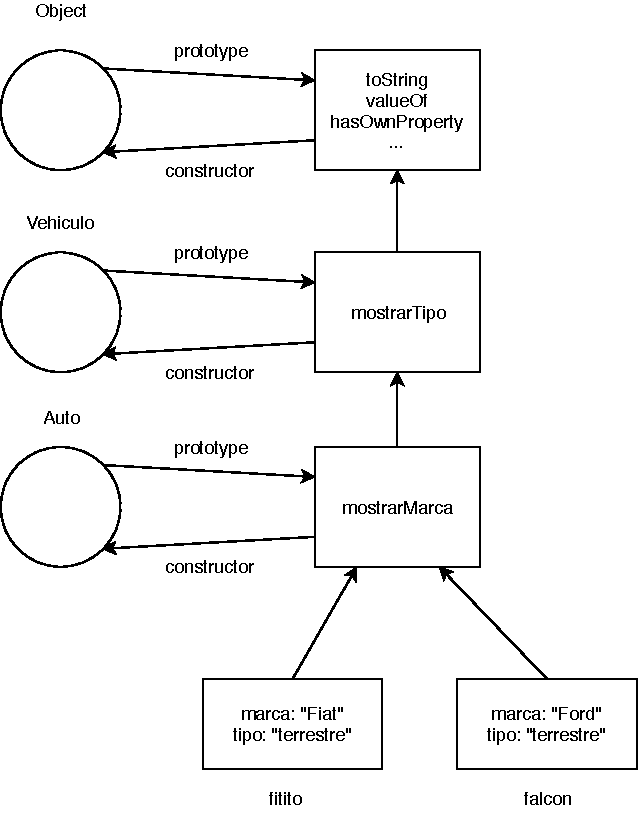
\includegraphics{Figures/Herencia}
\decoRule
\caption[Herencia prototipada]{Diagrama del código presentado}
\label{fig:herencia}
\end{figure}

\subsection{\code{extends} en ES6}

Tal como se explicó sobre la palabra reservada \code{class} en la sección \ref{clasesenes6}, otra de las características que se introdujeron a partir de la versión ES6 es la de la palabra \code{extends} para simular la herencia de clases. Nuevamente ocurre lo mismo que lo mencionado anteriormente: Esta característica es meramente \textit{syntactic sugar} que le omite al programador la necesidad de pensar en prototipos. 

\begin{lstlisting}[title={\code{extends} en ES6}]
class Vehiculo {
  constructor(tipo) {
    this.tipo = tipo;
  }
  mostrarTipo() {
    console.log(this.tipo);
  }
}

class Auto extends Vehiculo {
  constructor(marca) {
    super("terrestre");
    this.marca = marca;
  }
  mostrarMarca() {
    console.log(this.marca);
  }
}

var fitito = new Auto("Fiat");
var falcon = new Auto("Ford");
     
fitito.mostrarMarca();      // Fiat
fitito.mostrarTipo();       // terrestre

falcon.mostrarMarca();      // Ford
falcon.mostrarTipo();       // terrestre
\end{lstlisting}

Para el programador que viene de C++ o Java, este uso de \code{class} y \code{extends} es, por lejos, muchísimo más amigable que crear funciones y vincularlas mediante sus prototipos. Otra de las introducciones a partir de ES6 es el uso del \code{super} en el constructor. Esto facilita enormemente la llamada al constructor de la superclase, o de métodos de la superclase, además de mimetizar la sintaxis de Java. 

\subsection{Herencia múltiple}

Dado que los objetos "`heredan"' de un único prototipo, el lenguaje no provee ninguna herramienta natural para el soporte de la herencia múltiple. Otros lenguajes buscan alcanzar la herencia múltiple mediante el uso de interfaces. En JavaScript no existen las interfaces, pero sí existe una técnica llamada mixins (acrónimo para \textit{mixed in}, del inglés "`mezclado"') para introducir un comportamiento a una clase sin necesidad de hacerla heredar de otra.

Una función de Mixin suele tener esta forma:

\begin{lstlisting}[title={Función de Mixin}]
function mixin(fuente, destino) {  
  for (var prop in fuente) {
    if (fuente.hasOwnProperty(prop)) {
      destino[prop] = fuente[prop];
    }
  }
}
\end{lstlisting}

Lo ideal sería pensar en \code{fuente} como un objeto cuyas propiedades serán los miembros a "`inyectar"' en \code{destino}. Esta técnica llevó al estándar a agregar un método \code{Object.assign} a partir de ES6, el cual copia los valores de todas las propiedades enumerables en un objeto destino.

Otra manera de implementar los Mixins en ES6 es aprovechando que las clases son de primer órden. Éstas pueden ser pasadas como argumento o ser retornadas por una función.

\begin{lstlisting}[title={Haciendo uso de \code{class} como expresión}]
var MyMixin = (superclass) => class extends superclass {  
  saludar() {
    console.log('hola!');
  }
};

class Foo {}
class Bar extends MyMixin(Foo) {
  despedirse() {
    console.log('chau!');
  }
}

var objeto = new Bar();

objeto.saludar();			// hola!
objeto.despedirse();	// chau!
\end{lstlisting}

Como se puede observar, existen varias formas de aplicar esta técnica. Como se mencionó anteriormente, no hay soporte para herencia múltiple en JavaScript, aunque ésta es una forma de resolver el problema. Aún así, tiene sus defectos. El \textit{shadowing} u \textit{overriding} de métodos con el mismo identificador es una convención a tener en cuenta. También hay que pensar en el costo, ya que copiar las propiedades de un objeto a otro requiere de un esfuerzo.

\section{Encapsulamiento}

Dependiendo la perspectiva, se puede decir que el lenguaje tampoco provee un mecanismo natural para el encapsulamiento. Si hablamos de ocultar el estado de un objeto, es decir, de hacer sus datos miembro privados, no existe ninguna palabra reservada para ello. De hecho, todas las propiedades de un objeto son públicas.

Existe una convención extra oficial de que los miembros privados de un objeto comiencen su identificador con un guión bajo. Nuevamente, ésta no es una convención del lenguaje, sino de la comunidad. Más allá de la convención, volvemos a lo mismo: Por fuera se puede analizar cuál es el valor ligado a dicha propiedad.

\begin{lstlisting}[title={Descubriendo variables "`privadas"'}]
class Persona {
  constructor(nombre, saldo) {
    this.nombre = nombre;
    this._saldo = saldo;
  }
}

var pepe = new Persona('Jose', 25);

console.log(pepe.nombre);	// Jose
console.log(pepe._saldo);	// 25
\end{lstlisting}

Como se puede observar en el ejemplo, se busca hacer privada la propiedad \code{\_saldo}, pero sin embargo es visible desde afuera del objeto.

Por suerte mediante el uso de \textit{closures}, se puede lograr el encapsulamiento, pero solo mediante el uso de funciones constructoras. Lamentablemente, para la sintaxis de \code{class} de ES6 no hay soporte nativo aún. Al momento de escribirse este documento, existe una propuesta en borrador para agregar al lenguaje, la cual se encuentra en \textit{Stage 3} (para más información, ver \href{https://github.com/tc39/proposal-class-fields#private-fields}{https://github.com/tc39/proposal-class-fields\#private-fields}).

\begin{lstlisting}[title={Alcanzando variables privadas mediante closures}]
function Persona(nombre, saldo) {
  var saldoPrivado = saldo;
  this.nombre = nombre;
  this.obtenerSaldo = function() {
    return saldoPrivado;
  }
  this.actualizarSaldo = function(nuevoSaldo) {
    saldoPrivado = nuevoSaldo;
  }
}

var pepe = new Persona('Jose', 25);

console.log(pepe.nombre);					// Jose
console.log(pepe.saldoPrivado);		// undefined
// OK, ya que es una propiedad privada.
console.log(pepe.obtenerSaldo());	// 25
pepe.actualizarSaldo(32);
console.log(pepe.obtenerSaldo());	// 32
\end{lstlisting}

Un detalle menos obvio pero aún así importante, es que necesariamente los \textit{setters} y \textit{getters} de las variables ocultas por el closure deberán formar parte de la función constructora (es decir, no podrán definirse dentro del prototipo), lo que significa nuevamente que cada instancia de \code{Persona} tendrá código repetido, lo que implica gasto en memoria. Bajo esta situación, nos encontramos en un \textit{trade-off} de tener datos miembro privados, pero no poder hacer uso correcto del patrón prototipal.


\section{Polimorfismo}

Quizás uno de los puntos más complicados de analizar en cuanto a JavaScript y su relación con el paradigma de orientación a objetos sea el de polimorfismo, dado que por su naturaleza de débilmente tipado y su particularidad de herencia prototipada, no resultará simple hacer una comparación con lenguajes como C++ o Java. 

Para el caso de las funciones "`polimórficas"' el lenguaje no pone restricciones en relación a la aridad ni el tipo de los parámetros. Si la cantidad de argumentos dados al momento de una invocación es menor a la cantidad de parámetros formales de la función, entonces los restantes se considerarán con valor \code{undefined}. 

Existe un identificador especial reservado para el vector de argumentos en JavaScript, bajo el identificador de \code{arguments}. Este es un objeto especial, aunque a simple vista parece un arreglo, no lo es. Funciona de una forma similar a lo que es \code{args} en Java o \code{argv} en C++. Supongamos a continuación una función que no tiene definidos parámetros formales, pero aún así recibe argumentos a la hora de invocarla.

\begin{lstlisting}[title={Analizando \code{arguments}}]
function mostrarArgumentos() {
  for (var i = 0; i < arguments.length; i++) {
    console.log(i + ". " + arguments[i]);
  }
}

mostrarArgumentos("hola", 1, true, { a: 3 });

// 0. hola
// 1. 1
// 2. true
// 3. [object Object]
\end{lstlisting}

Para el caso de polimorfismo bajo una misma jerarquía de herencia, dado que el lenguaje es débilmente tipado, no posee las restricciones fuertes que posee un lenguaje como Java. Al ser interpretado, no existe un chequeo estático para corroborar que un método que esté siendo invocado pertenezca a un tipo o una clase particular. Ésta característica, la de redefinir un método de la superclase en una subclase, se llama polimorfismo de inclusión (o de subtipado).

\begin{lstlisting}
class Animal {
	mover() {}
}
class Pez extends Animal {
  mover() {
    console.log("Soy pez y estoy nadando...");
  }
}
class Ave extends Animal {
  mover() {
    console.log("Soy ave y estoy volando...");
  }
}

var animales = [new Pez(), new Ave()];

for (let animal of animales) {
  animal.mover();
}

// Soy pez y estoy nadando...
// Soy ave y estoy volando...
\end{lstlisting}

?`Qué sucede exactamente?. En ejecución, cada elemento de la lista de \code{animales} hará búsqueda del método \code{mover} en su cadena de prototipo. En caso de no encontrarlo, resultará en un error en ejecución. 

\section{Modularidad}
\label{sec:modulos}

Durante sus primeros 20 años de vida, JavaScript no proveía soporte para módulos de una forma nativa. En 2015 con la salida de ES6, el lenguaje adquirió ese soporte nativo que le faltaba. Sin embargo, aún no todos los navegadores (o motores) soportan todas las funcionalidades introducidas en ES6 y las nuevas versiones del estándar.

En ésta sección vamos a mencionar cuáles son las formas en las que se alcanza la modularidad en JavaScript.

\subsection{Módulos mediante patrones}

Al igual que sucede con las clases, se hace el uso de IIFE y closures para aplicar patrones conocidos en la creación de módulos. El patrón por excelencia en este caso es el Revealing Module pattern. Si este patrón es implementado mediante IIFE, se lo puede pensar al módulo como un singleton, ya que al momento de definir el módulo se está creando una única instancia del mismo.

\begin{lstlisting}[title={Revealing module pattern}]
var ModuloSaludador = (function () {
  var cantidadSaludos = 0;

  var incrementarSaludos = function() {
    cantidadSaludos++;
  }

  var saludar = function() {
    console.log("hola");
    incrementarSaludos();
  }

  var despedirse = function() {
    console.log("chau");
    incrementarSaludos();
  }

  var mostrarContador = function() {
    console.log(cantidadSaludos);
  }

  return {
    saludar: saludar,
    despedirse: despedirse,
    imprimirEstado: mostrarContador
  }
}());

ModuloSaludador.saludar();				// hola
ModuloSaludador.despedirse();			// chau
ModuloSaludador.imprimirEstado();	// 2
\end{lstlisting}

Para el ejemplo dado, se mantiene un estado interno que cuenta la cantidad de saludos dados. Se puede apreciar como tanto \code{cantidadSaludos} y la función \code{incrementarSaludos} son de alguna forma atributos privados del módulo. 

Lo que retorna la función constructora del módulo en realidad es un objeto con las funciones del mismo, a modo de API. Notar el detalle de la función \code{mostrarContador}, que internamente para el módulo se llamará de esa manera, pero el módulo la expone con otro nombre, \code{imprimirEstado}.

La simplicidad de éste método de modularizar es una gran ventaja. No se requieren librerías externas. Una ventaja clara de la utilización de módulos es que podemos mantener \code{namespaces} más limpios a nivel aplicación.

Una desventaja de éste método es que no existe un manejo de dependencias entre módulos. Se puede hacer inyección de dependencias pasándole mediante parámetro el módulo que queremos inyectar como dependencia al nuevo módulo que estemos definiendo. Esto nos obliga a tener que pensar qué módulos deben estar definidos previamente a otros (recordar que el módulo es una IIFE), o nos obliga a cambiar un poco el patrón y utilizar algo más similar al Prototype class pattern, en donde podremos crear más de una instancia de un módulo en particular. Veremos en las soluciones siguientes cómo se aborda el manejo de dependencias para las otras técnicas.

\subsection{Sistemas de módulos}

Ante la falta de soporte, la propia comunidad se encargó de crear sus propios formatos estandarizados para modularizar sus aplicaciones. A mi entender, las dos partes claves que se agregaron con esta solución fue el manejo de dependencias entre módulos, y la capacidad de poder separar módulos en distintos archivos.

Los dos formatos más populares son \keyword{AMD} y \keyword{CommonJS}. Se pueden pensar a estos formatos como la parte sintáctica de los módulos, ya que luego será necesario hacer uso de algún module loader (librerías externas tales como \keyword{SystemJS} o \keyword{RequireJS}) para conectar y hacer funcionar a los módulos.

\subsubsection{AMD}

La sigla representa "`Asynchronous Module Definition"', en español sería definición de módulo asíncrono. Tal como se puede intuir por el nombre, se trata de una especificación para definir módulos y dependencias, y que las mismas sean cargadas de forma asincrónica.

En la especificación se puede encontrar un único método \code{define} para definir un módulo que, tiene sus variantes dependiendo de la cantidad y el tipo de los parámetros dados. Para los ejemplos que se mencionarán aquí, solo usaremos dos parámetros: el primero, un \code{Array} que representan las dependencias del módulo que estamos definiendo, y el segundo, una \code{Function} que será la definición del módulo propiamente dicho.
% https://github.com/amdjs/amdjs-api/blob/master/AMD.md 

Un ejemplo de módulo con dependencias podría ser el siguiente:

\begin{lstlisting}[title={Ejemplo de AMD}]
define(['./math', './mailer'], function (math, mailer) {
  var enviarSiEsPrimo = function(n, email) {
    if (math.esPrimo(n)) {
      mailer.enviar(email);
    }
  }

  return {
    enviarSiEsPrimo: enviarSiEsPrimo
  }
})
\end{lstlisting}

El primer parámetro dado es un arreglo con las dependencias. En nuestro caso, damos la ruta relativa a otros dos módulos \textit{math} y \textit{mailer} que supongamos que existen. El segundo parámetro es la definición del módulo que queremos crear, el cual será una función cuyos argumentos formales corresponden a las dos dependencias recién mencionadas. Lo que sucede por detrás es una inyección de éstas dependencias. 

Para nuestro caso del ModuloContador, una adaptación en AMD podría ser la siguiente:

\begin{lstlisting}[title={Modulo contador en AMD}]
define([], function () {
  var cantidadSaludos = 0;

  var incrementarSaludos = function() {
    cantidadSaludos++;
  }

  var saludar = function() {
    console.log("hola");
    incrementarSaludos();
  }

  var despedirse = function() {
    console.log("chau");
    incrementarSaludos();
  }

  var mostrarContador = function() {
    console.log(cantidadSaludos);
  }

  return {
    saludar: saludar,
    despedirse: despedirse,
    imprimirEstado: mostrarContador
  };
});
\end{lstlisting}

\subsubsection{CommonJS}

La otra especificación de módulos popular es la de CommonJS. A diferencia de AMD, la carga de los módulos se hace de forma sincrónica.

Podemos separar a la definición de un módulo en tres partes:
\begin{itemize}
	\item La importación de las dependencias, que se hacen mediante un método especial \code{require}.
	\item La definición del módulo propiamente dicho, es decir, su código.
	\item La exportación de los métodos públicos del módulo, mediante uso de la propiedad \code{module.exports}.
\end{itemize}

Nuevamente, la idea no es profundizar sobre la especificación de CommonJS. De hecho, es un poco más amplia de lo que se menciona en éste documento, pero para el concepto que se quiere mostrar, es suficiente con lo recién mencionado.

Un ejemplo equivalente a lo realizado en el módulo AMD, el cual usaba dependencias \textit{math} y \textit{mailer}, podría ser el siguiente:

\begin{lstlisting}
var math = require('./math');
var mailer = require('./mailer');

var enviarSiEsPrimo = function(n, email) {
  if (math.esPrimo(n)) {
    mailer.enviar(email);
  }
};

module.exports.enviarSiEsPrimo = enviarSiEsPrimo;
\end{lstlisting}

Para el caso del ModuloContador, una versión en CommonJS podría ser la siguiente:

\begin{lstlisting}[title={Modulo contador en CommonJS}]
var cantidadSaludos = 0;

var incrementarSaludos = function() {
  cantidadSaludos++;
};

var saludar = function() {
  console.log('hola');
  incrementarSaludos();
};

var despedirse = function() {
  console.log('chau');
  incrementarSaludos();
};

var mostrarContador = function() {
  console.log(cantidadSaludos);
};

module.exports = {
  saludar: saludar,
  despedirse: despedirse,
  imprimirEstado: mostrarContador
};
\end{lstlisting}

\subsection{Módulos	en ES6}

Probablemente una de las características más enriquecedoras introducidas a partir de ES6, es la del soporte nativo para los módulos. Este soporte de módulos mimetiza la característica de asincronía en AMD, y la sintaxis concisa en CommonJS. De hecho, la sintaxis es extramadamente más concisa que en CommonJS, además de que se tiene un mejor soporte para las dependencias cíclicas, y gracias a la estructura de los módulos en ES6, se puede hacer un análisis estático y así realizar, por ejemplo, optimizaciones.

Las dos palabras resevadas a tener en cuenta para éste tipo de modularización son \code{import} y \code{export}. Con \code{import} se realizará la importación de dependencias para el módulo que estemos definiendo. Con \code{export}, se realizará la exportación cualquier miembro del módulo que se desee exponer. Una vez más, existen variantes para la parte de \code{export} como por ejemplo \textit{named export} y \textit{default export} que si bien se las mencionarán mediante ejemplos, escapan de este documento y queda a cargo del lector conocerlas en detalle.

Un dato a tener en cuenta, es que el soporte de los módulos para ES6 aún no está implementado en su completitud en el intérprete de todos los navegadores. Al punto tal de que quizás para hacer uso de ésta característica puede que sea necesaria una herramienta de traducción y compilación (acción conocida como "`transpile"') tal como \keyword{Babel}, y una herramienta de compilación o empaquetamiento tal como \keyword{Webpack}.

Tomando como caso de ejemplo el supuesto módulo \textit{math} visto en las secciones anteriores, podríamos hacer \code{import} de éste módulo dependiendo de la forma en la que se esté exportando.

\begin{lstlisting}[title={Algunos ejemplos de \code{import}}]
// importando lo que esté por "default" 
import math from './math';
// importando todo lo exportado por math
import * as math from './math';
// importando y haciendo destructuring de lo que nos sirva
import { esPrimo } from './math'
\end{lstlisting}

Para el caso de la exportación también existen varias maneras, y dependiendo de cuál se utilice, será correspondiente luego la forma en la que se importe.

\begin{lstlisting}[title={Algunos ejemplos de \code{export}}]
// exportando una constante con nombre
export const PI = 3.1416;
// exportando una funcion
export function foo() { console.log('foo') }
// exportando con "default"
export default function bar() {}
\end{lstlisting}

Dependiendo cual sea el caso, tiene sentido después pensar qué parte del módulo se está importando: Si tan solo una parte, el módulo completo, alguna función o atributo particular (siempre que se esté exportando), o lo que exporta el módulo por defecto.

Siguiendo con el grupo de ejemplos, se muestra cómo sería una implementación en ES6 de los módulos ejemplificados en las secciones anteriores:

\begin{lstlisting}[title={Ejemplo de módulo en ES6}]
import { esPrimo } from './math';
import { enviar } from './mailer';

export function enviarSiEsPrimo(n, email) {
  if (esPrimo(n)) {
    enviar(email);
  }
}
\end{lstlisting}

Una particularidad a tener en cuenta en este ejemplo es que en las lineas 1 y 2 se hizo \textit{destructuring} de los módulos \textit{math} y \textit{mailer}, dado que solo nos interesan las funciones \code{esPrimo} y \code{enviar}. Por otro lado, el \code{export} en la definición de la función se puede hacer de forma separada (es decir, definir la función por un lado y luego hacer \code{export enviarSiEsPrimo}. Cualquiera de las dos formas es válida, pero se busca mostrar qué tan conciso queda el código con ES6.

Ahora veamos un ejemplo de ModuloContador, el cual no posee dependencias. Para este caso, mostraremos una variante del \code{export} totalmente válida, en la que se hace un único \code{export} de las tres funciones que expone el módulo.

\begin{lstlisting}[title={Modulo contador en ES6}]
var cantidadSaludos = 0;

var incrementarSaludos = function() {
  cantidadSaludos++;
};

var saludar = function() {
  console.log('hola');
  incrementarSaludos();
};

var despedirse = function() {
  console.log('chau');
  incrementarSaludos();
};

var mostrarContador = function() {
  console.log(cantidadSaludos);
};

export { saludar, despedirse, mostrarContador as imprimirEstado };
\end{lstlisting}

\section{Conclusiones}

\begin{itemize}
\item Lo bueno: 
La herencia prototipal y su poder. El modelo de delegación de comportamiento y la cadena de prototipo, y la falta de necesidad de copiar o guardar lugar en memoria para los miembros de la superclase seguramente lo hacen más liviano. 
La sintaxis de clase de ES6 fue probablemente una de las mejores características lanzadas para el lenguaje. Permite a muchos programadores meterse en el lenguaje sin necesidad de cambiarles la mentalidad de herencia clásica a la prototipal.
Dicho todo esto, JavaScript es un verdadero lenguaje orientado a objetos, mientras que otros lenguajes son orientados a clases.
El polimorfismo (o en realidad la falta de chequeos en "`compilación"') es otro punto a destacar. Le saca rigurosidad (y seguridad) al lenguaje incrementando su flexibilidad. Si quiero invocar a un método de un objeto y éste no existe, se buscará en la cadena de prototipo hasta terminar con la cadena, y en caso de que así sea, habrá un error en ejecución.
Otra característica que también merece una mención es la de los módulos de ES6, ya que de una manera clara y concisa se pueden separar espacios de nombres y manejar las dependencias sin la necesidad de pensar en ellas.
\item Lo malo: 
La falta de soporte natural para las clases es algo que deja que desear del lenguaje. Para ser justos con él, no fue pensado para tener clases (y es por eso que no tiene herencia clásica), y aún así los programadores buscan llegar a las mismas. Sin embargo, el soporte dado a las clases en ES6 es únicamente sintáctico, y el estándar parece estar conforme con dichas bases como para seguir evolucionando en éste punto. 
La asignación "`manual"' del prototipo de una función al querer simular la herencia clásica es un arma de doble filo, ya que si bien nos da libertades, es muy fácil perderse entre las relaciones que hay entre los objetos. Por otro lado, la poca popularidad de la herencia prototipal hace de JavaScript un lenguaje más difícil de comprender.
\item Lo feo: 
No poder poseer miembros privados, ya sean atributos o funciones, y tener que recurrir a aplicar mecanismos como closures e IIFEs para alcanzar esto. Todos los métodos y los atributos cargados en un objeto serán públicos y habrá que pensar en un buen diseño de aplicación para no tener problema con ello. Por suerte, los módulos de ES6 solucionan una parte de esto, ya que de forma implícita, los métodos que no se exporten en un módulo valdrán como métodos privados para ese módulo.
\end{itemize}


\chapter{Conclusión: Parte II}

\section{Lo bueno}

Por parte del paradigma de programación funcional, JavaScript no será un lenguaje de programación funcional pura, pero el hecho de que las funciones sean valores dentro del lenguaje lo hace excesivamente poderoso. Poseer funciones como valores, permitir el paso de las mismas como argumentos o como valores de retorno hace al lenguaje sumamente expresivo.

Para la enseñanza de conceptos básicos de la programación funcional, con una sintaxis similar a la familia de lenguajes de C, es un buen lenguaje, más allá de la falta de todas las propiedades que corresponden a un lenguaje 100\% del paradigma funcional.

Por el lado del paradigma de orientación a objetos, la herencia prototipal es una de las características destacadas. El modelo de delegación de comportamiento y la cadena de prototipo, y la falta de necesidad de copiar o guardar lugar en memoria para los miembros de la superclase seguramente lo hacen más liviano, pero a su vez con un extremo poder.
 
La sintaxis de clase de ES6 fue probablemente una de las mejores características lanzadas para el lenguaje. Permite a muchos programadores meterse en el lenguaje sin necesidad de cambiarles la mentalidad de herencia clásica a la prototipal. La incorporación de la sintaxis de \code{class} y \code{extends} fue sin dudas, un acierto.

En el sentido de la programación "`orientada a \textit{objetos}"', JavaScript es un verdadero lenguaje orientado a objetos, mientras que otros lenguajes son orientados a \textit{clases}. Volvemos a insistir sobre un algo marcado anteriormente: \textit{Casi todo en JavaScript es un objeto}: Funciones, arreglos, clases y módulos.

El polimorfismo (o en realidad la falta de chequeos en "`compilación"') es otro punto a destacar. Le saca rigurosidad al lenguaje incrementando su flexibilidad. Si se desea invocar a un método de un objeto y éste no existe, se buscará en la cadena de prototipo hasta terminar con la cadena, y en caso de que así sea, habrá un error en ejecución.

Una característica que también merece una mención es la de los módulos de ES6, ya que de una manera clara y concisa se pueden separar espacios de nombres y manejar las dependencias sin la necesidad de pensar en ellas.

\section*{Lo malo}

Algunas carencias tales como la falta de evaluación perezosa, semántica de valores y transparencia referencial, alejan a JavaScript del paradigma funcional. A pesar de ello, si tuviera éstas características seguramente tendríamos que limitar al lenguaje en otros aspectos, y probablemente quitarle el soporte para otros paradigmas de programación. Si vamos al caso, agregar semántica de valores y transparencia referencial implica perder la noción de "`estado"', por lo que éste acercamiento al paradigma funcional nos obligaría a alejarnos del paradigma orientado a objetos.

Por el lado del paradigma de orientación a objetos, la falta de soporte natural para las clases es algo que deja que desear del lenguaje. Para ser justos con él, no fue pensado para tener clases (y es por eso que no tiene herencia clásica), y aún así los programadores buscan llegar a las mismas. No obstante, el soporte dado a las clases en ES6 es únicamente sintáctico, y el estándar parece estar conforme con dichas bases como para seguir evolucionando en éste punto. 

La asignación "`manual"' del prototipo de una función al querer simular la herencia clásica es un arma de doble filo, ya que si bien nos da libertades, es muy fácil perderse entre las relaciones que hay entre los objetos. Por otro lado, la poca popularidad de la herencia prototipal hace de JavaScript un lenguaje más difícil de comprender.
\section{Lo feo}

Por el lado del paradigma funcional, si existiera un constructor natural para que los valores sean inmutables, servirían de extrema ayuda para acercarse aún más a dicho paradigma. Lamentablemente ésto no existe, entonces si queremos acercarnos a la programación funcional mediante JavaScript, tenemos que hacer uso de librerías externas.

Una de las características desagradables con respecto al paradigma orientado a objetos, es la falta de miembros privados, ya sean atributos o funciones, y tener que recurrir a aplicar mecanismos como closures e IIFEs para alcanzar esto. Todos los métodos y los atributos cargados en un objeto serán públicos y habrá que pensar en un buen diseño de aplicación para no tener problema con ello. Por suerte, los módulos de ES6 solucionan una parte de esto, ya que de forma implícita, los métodos que no se exporten en un módulo valdrán como métodos privados para ese módulo.

% CIERRE
\chapter{Conclusiones generales}

A modo de cierre, en el siguiente capítulo se presentan algunas características o conceptos que no fueron tratados en el documento pero que es necesario marcarle al lector, en caso de que quisiera seguir profundizando sobre JavaScript. Para terminar, se expondrán conclusiones generales de la tesis, volcando una opinión que se fue formando durante el proceso de investigación del lenguaje. 

\section{A futuro}

Las características del lenguaje vistas en éste documento solo forman parte de un subconjunto del lenguaje. De hecho, existen muchísimos otros aspectos para analizar del lenguaje. A continuación se le presentan al lector algunos términos que son dignos de destacar, en caso de que se quisiera seguir profundizando en el área:

\begin{itemize}
\item \keyword{Nuevas características sintácticas de ES6}: A partir de las nuevas versiones del estándar se introdujeron nuevos conceptos que facilitan la tarea del programador. Template literals, Spread y Rest operators, Default values, Destructuring
\item \keyword{Otros conceptos de ES6}: No solo se introdujeron características sintácticas en ES6, sino que aparecieron clases que son de ayuda para la \textit{meta-programación}, como por ejemplo: Symbol, Proxy, Iterators, Generators.
\item \keyword{Concurrencia}: JavaScript es un lenguaje \textit{single thread} y su fortaleza yace en el \textit{event loop}, del cual no se ha hablado en éste documento, pero es un concepto clave para entender cómo ese \textit{único hilo} maneja la concurrencia.
\item \keyword{Asincronía}: Directamente relacionado con el ítem anterior, se puede investigar sobre cómo se maneja la asincronía en JavaScript. Algunos conceptos destacables son: Callbacks, Promises, Generators, \code{await} y \code{async}.
\end{itemize}
\section{Resumen}

JavaScript es expresivo y a su vez es sintácticamente agradable. Tiene facilidad para la escritura de programas, pero habiendo tantas combinaciones entre los constructores, la facilidad de lectura dependerá de la experiencia del programador. De alguna forma también es conciso en cuanto a la cantidad de líneas de código que se necesitan para hacer un programa.

Con un sistema de tipos extremadamente flexible, la seguridad en su sistema de tipos se ve reducida, ya que la coerción en ciertas expresiones pueden llevar a resultados inesperados. En este sentido, la confiabilidad del lenguaje se ve directamente afectada. 

Está claro que JavaScript es un lenguaje de "`scripting"' pero a su vez es multi-paradigma. Con un esfuerzo mediano, se aproxima a la idea del paradigma funcional tanto como a la del paradigma de orientación a objetos. Si bien es imposible que alcance la pureza en ambos de forma simultánea, la cobertura que le da a ambos paradigmas es aceptable.

Uno de los mayores problemas del lenguaje es su nombre. Hacer creer a los programadores que por llamarse JavaScript tendrá similitudes con Java es totalmente errado. De hecho, como se presentó en el documento, la semántica de ambos lenguajes están lejos una de otra.

El lenguaje tiene varios \textit{bugs}, es cierto, y eso no se puede negar. Teniéndole un poco de piedad al lenguaje, se puede decir que el mismo se "`creó en 10 días"', sin embargo tardó 20 años en agregar características que realmente eran necesarias para los programadores. 

No podemos afirmar que JavaScript es un lenguaje popular por sus características técnicas. Más bien, la popularidad probablemente se haya obtenido por factores externos, como la voluntad de su comunidad, o cuestiones empresariales o de mercado. Sin embargo, el gran acierto de JavaScript fue haber dado el "`primer golpe"' en la rama de la programación web. Cuesta imaginarse qué hubiera sido del lenguaje si éste no hubiera sido el pionero.

Lo esperanzador para el lenguaje es que después del lanzamiento de Node en 2009, más su actualización en la especificación en el año 2015, la comunidad creció de manera exponencial. No solo eso, se alienta a los programadores para que ellos mismos sean los que suban propuestas del lenguaje. En los últimos cuatro años, el estandar de ECMAScript se ha actualizado en Junio cada año. En este sentido, el lenguaje pareciera que seguirá evolucionando.

Para concluir, es necesario llamar a la reflexión del lector: \textit{El lenguaje es sólamente una herramienta}. Está en cáda uno de qué forma y para qué utiliza dicha "`herramienta"'.

%----------------------------------------------------------------------------------------
%	THESIS CONTENT - APPENDICES
%----------------------------------------------------------------------------------------

%\appendix % Cue to tell LaTeX that the following "chapters" are Appendices

% Include the appendices of the thesis as separate files from the Appendices folder
% Uncomment the lines as you write the Appendices

%% Appendix A

\chapter{Frequently Asked Questions} % Main appendix title

\label{AppendixA} % For referencing this appendix elsewhere, use \ref{AppendixA}

\section{How do I change the colors of links?}

The color of links can be changed to your liking using:

{\small\verb!\hypersetup{urlcolor=red}!}, or

{\small\verb!\hypersetup{citecolor=green}!}, or

{\small\verb!\hypersetup{allcolor=blue}!}.

\noindent If you want to completely hide the links, you can use:

{\small\verb!\hypersetup{allcolors=.}!}, or even better: 

{\small\verb!\hypersetup{hidelinks}!}.

\noindent If you want to have obvious links in the PDF but not the printed text, use:

{\small\verb!\hypersetup{colorlinks=false}!}.

%\include{Appendices/AppendixB}
%\include{Appendices/AppendixC}

%----------------------------------------------------------------------------------------
%	BIBLIOGRAPHY
%----------------------------------------------------------------------------------------

\nocite{*}
\printbibliography[heading=bibintoc]

%----------------------------------------------------------------------------------------

\end{document}  
